% !TEX root = main.tex
\section{Auswertung}
\label{sec:Auswertung}

\begin{figure}[ht]
    \centering
    % GNUPLOT: LaTeX picture with Postscript
\begingroup
  % Encoding inside the plot.  In the header of your document, this encoding
  % should to defined, e.g., by using
  % \usepackage[cp1252,<other encodings>]{inputenc}
  \inputencoding{cp1252}%
  \makeatletter
  \providecommand\color[2][]{%
    \GenericError{(gnuplot) \space\space\space\@spaces}{%
      Package color not loaded in conjunction with
      terminal option `colourtext'%
    }{See the gnuplot documentation for explanation.%
    }{Either use 'blacktext' in gnuplot or load the package
      color.sty in LaTeX.}%
    \renewcommand\color[2][]{}%
  }%
  \providecommand\includegraphics[2][]{%
    \GenericError{(gnuplot) \space\space\space\@spaces}{%
      Package graphicx or graphics not loaded%
    }{See the gnuplot documentation for explanation.%
    }{The gnuplot epslatex terminal needs graphicx.sty or graphics.sty.}%
    \renewcommand\includegraphics[2][]{}%
  }%
  \providecommand\rotatebox[2]{#2}%
  \@ifundefined{ifGPcolor}{%
    \newif\ifGPcolor
    \GPcolorfalse
  }{}%
  \@ifundefined{ifGPblacktext}{%
    \newif\ifGPblacktext
    \GPblacktexttrue
  }{}%
  % define a \g@addto@macro without @ in the name:
  \let\gplgaddtomacro\g@addto@macro
  % define empty templates for all commands taking text:
  \gdef\gplbacktext{}%
  \gdef\gplfronttext{}%
  \makeatother
  \ifGPblacktext
    % no textcolor at all
    \def\colorrgb#1{}%
    \def\colorgray#1{}%
  \else
    % gray or color?
    \ifGPcolor
      \def\colorrgb#1{\color[rgb]{#1}}%
      \def\colorgray#1{\color[gray]{#1}}%
      \expandafter\def\csname LTw\endcsname{\color{white}}%
      \expandafter\def\csname LTb\endcsname{\color{black}}%
      \expandafter\def\csname LTa\endcsname{\color{black}}%
      \expandafter\def\csname LT0\endcsname{\color[rgb]{1,0,0}}%
      \expandafter\def\csname LT1\endcsname{\color[rgb]{0,1,0}}%
      \expandafter\def\csname LT2\endcsname{\color[rgb]{0,0,1}}%
      \expandafter\def\csname LT3\endcsname{\color[rgb]{1,0,1}}%
      \expandafter\def\csname LT4\endcsname{\color[rgb]{0,1,1}}%
      \expandafter\def\csname LT5\endcsname{\color[rgb]{1,1,0}}%
      \expandafter\def\csname LT6\endcsname{\color[rgb]{0,0,0}}%
      \expandafter\def\csname LT7\endcsname{\color[rgb]{1,0.3,0}}%
      \expandafter\def\csname LT8\endcsname{\color[rgb]{0.5,0.5,0.5}}%
    \else
      % gray
      \def\colorrgb#1{\color{black}}%
      \def\colorgray#1{\color[gray]{#1}}%
      \expandafter\def\csname LTw\endcsname{\color{white}}%
      \expandafter\def\csname LTb\endcsname{\color{black}}%
      \expandafter\def\csname LTa\endcsname{\color{black}}%
      \expandafter\def\csname LT0\endcsname{\color{black}}%
      \expandafter\def\csname LT1\endcsname{\color{black}}%
      \expandafter\def\csname LT2\endcsname{\color{black}}%
      \expandafter\def\csname LT3\endcsname{\color{black}}%
      \expandafter\def\csname LT4\endcsname{\color{black}}%
      \expandafter\def\csname LT5\endcsname{\color{black}}%
      \expandafter\def\csname LT6\endcsname{\color{black}}%
      \expandafter\def\csname LT7\endcsname{\color{black}}%
      \expandafter\def\csname LT8\endcsname{\color{black}}%
    \fi
  \fi
    \setlength{\unitlength}{0.0500bp}%
    \ifx\gptboxheight\undefined%
      \newlength{\gptboxheight}%
      \newlength{\gptboxwidth}%
      \newsavebox{\gptboxtext}%
    \fi%
    \setlength{\fboxrule}{0.5pt}%
    \setlength{\fboxsep}{1pt}%
\begin{picture}(7200.00,5040.00)%
    \gplgaddtomacro\gplbacktext{%
      \csname LTb\endcsname%%
      \put(682,704){\makebox(0,0)[r]{\strut{}$0$}}%
      \put(682,1161){\makebox(0,0)[r]{\strut{}$2$}}%
      \put(682,1618){\makebox(0,0)[r]{\strut{}$4$}}%
      \put(682,2076){\makebox(0,0)[r]{\strut{}$6$}}%
      \put(682,2533){\makebox(0,0)[r]{\strut{}$8$}}%
      \put(682,2990){\makebox(0,0)[r]{\strut{}$10$}}%
      \put(682,3447){\makebox(0,0)[r]{\strut{}$12$}}%
      \put(682,3905){\makebox(0,0)[r]{\strut{}$14$}}%
      \put(682,4362){\makebox(0,0)[r]{\strut{}$16$}}%
      \put(682,4819){\makebox(0,0)[r]{\strut{}$18$}}%
      \put(814,484){\makebox(0,0){\strut{}$1400$}}%
      \put(1479,484){\makebox(0,0){\strut{}$1500$}}%
      \put(2145,484){\makebox(0,0){\strut{}$1600$}}%
      \put(2810,484){\makebox(0,0){\strut{}$1700$}}%
      \put(3476,484){\makebox(0,0){\strut{}$1800$}}%
      \put(4141,484){\makebox(0,0){\strut{}$1900$}}%
      \put(4807,484){\makebox(0,0){\strut{}$2000$}}%
      \put(5472,484){\makebox(0,0){\strut{}$2100$}}%
      \put(6138,484){\makebox(0,0){\strut{}$2200$}}%
      \put(6803,484){\makebox(0,0){\strut{}$2300$}}%
    }%
    \gplgaddtomacro\gplfronttext{%
      \csname LTb\endcsname%%
      \put(209,2761){\rotatebox{-270}{\makebox(0,0){\strut{}Amplitude $\SI{\mycro \volt}$}}}%
      \put(3808,154){\makebox(0,0){\strut{}frequency in $\SI{\hertz}$}}%
      \csname LTb\endcsname%%
      \put(5816,4646){\makebox(0,0)[r]{\strut{}noisemagnitude spectrum}}%
    }%
    \gplbacktext
    \put(0,0){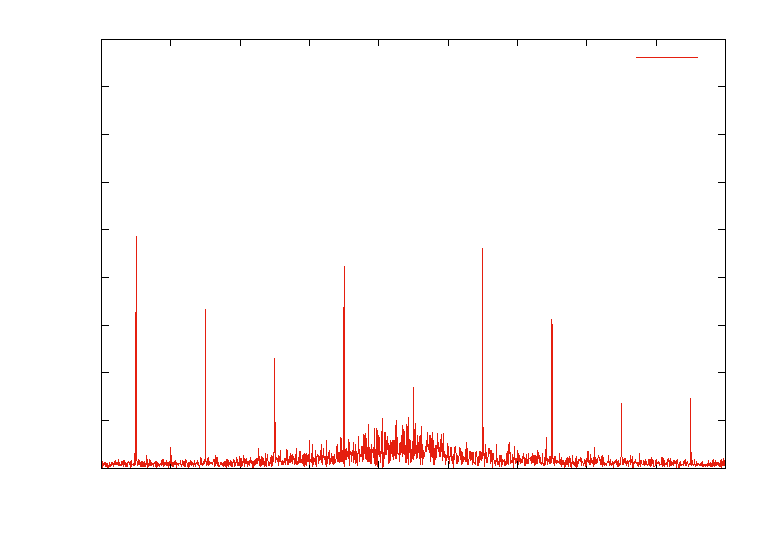
\includegraphics{plots/MonitorNoise13,8}}%
    \gplfronttext
  \end{picture}%
\endgroup

    \caption[]{13,8 Kapazität, schauen weil blöd 14.2 statt 13.8. Raischen nimmt nicht ab??????. Peaks aus stromquelle. Begründe 13.8 statt 14.2 da 7.5 mikrovolt statt 7.6. sowieso eh schon unter 10}
    \label{fig:MonitorNoise13,8}
\end{figure}

\begin{figure}[ht]
    \centering
    % GNUPLOT: LaTeX picture with Postscript
\begingroup
  % Encoding inside the plot.  In the header of your document, this encoding
  % should to defined, e.g., by using
  % \usepackage[cp1252,<other encodings>]{inputenc}
  \inputencoding{cp1252}%
  \makeatletter
  \providecommand\color[2][]{%
    \GenericError{(gnuplot) \space\space\space\@spaces}{%
      Package color not loaded in conjunction with
      terminal option `colourtext'%
    }{See the gnuplot documentation for explanation.%
    }{Either use 'blacktext' in gnuplot or load the package
      color.sty in LaTeX.}%
    \renewcommand\color[2][]{}%
  }%
  \providecommand\includegraphics[2][]{%
    \GenericError{(gnuplot) \space\space\space\@spaces}{%
      Package graphicx or graphics not loaded%
    }{See the gnuplot documentation for explanation.%
    }{The gnuplot epslatex terminal needs graphicx.sty or graphics.sty.}%
    \renewcommand\includegraphics[2][]{}%
  }%
  \providecommand\rotatebox[2]{#2}%
  \@ifundefined{ifGPcolor}{%
    \newif\ifGPcolor
    \GPcolorfalse
  }{}%
  \@ifundefined{ifGPblacktext}{%
    \newif\ifGPblacktext
    \GPblacktexttrue
  }{}%
  % define a \g@addto@macro without @ in the name:
  \let\gplgaddtomacro\g@addto@macro
  % define empty templates for all commands taking text:
  \gdef\gplbacktext{}%
  \gdef\gplfronttext{}%
  \makeatother
  \ifGPblacktext
    % no textcolor at all
    \def\colorrgb#1{}%
    \def\colorgray#1{}%
  \else
    % gray or color?
    \ifGPcolor
      \def\colorrgb#1{\color[rgb]{#1}}%
      \def\colorgray#1{\color[gray]{#1}}%
      \expandafter\def\csname LTw\endcsname{\color{white}}%
      \expandafter\def\csname LTb\endcsname{\color{black}}%
      \expandafter\def\csname LTa\endcsname{\color{black}}%
      \expandafter\def\csname LT0\endcsname{\color[rgb]{1,0,0}}%
      \expandafter\def\csname LT1\endcsname{\color[rgb]{0,1,0}}%
      \expandafter\def\csname LT2\endcsname{\color[rgb]{0,0,1}}%
      \expandafter\def\csname LT3\endcsname{\color[rgb]{1,0,1}}%
      \expandafter\def\csname LT4\endcsname{\color[rgb]{0,1,1}}%
      \expandafter\def\csname LT5\endcsname{\color[rgb]{1,1,0}}%
      \expandafter\def\csname LT6\endcsname{\color[rgb]{0,0,0}}%
      \expandafter\def\csname LT7\endcsname{\color[rgb]{1,0.3,0}}%
      \expandafter\def\csname LT8\endcsname{\color[rgb]{0.5,0.5,0.5}}%
    \else
      % gray
      \def\colorrgb#1{\color{black}}%
      \def\colorgray#1{\color[gray]{#1}}%
      \expandafter\def\csname LTw\endcsname{\color{white}}%
      \expandafter\def\csname LTb\endcsname{\color{black}}%
      \expandafter\def\csname LTa\endcsname{\color{black}}%
      \expandafter\def\csname LT0\endcsname{\color{black}}%
      \expandafter\def\csname LT1\endcsname{\color{black}}%
      \expandafter\def\csname LT2\endcsname{\color{black}}%
      \expandafter\def\csname LT3\endcsname{\color{black}}%
      \expandafter\def\csname LT4\endcsname{\color{black}}%
      \expandafter\def\csname LT5\endcsname{\color{black}}%
      \expandafter\def\csname LT6\endcsname{\color{black}}%
      \expandafter\def\csname LT7\endcsname{\color{black}}%
      \expandafter\def\csname LT8\endcsname{\color{black}}%
    \fi
  \fi
    \setlength{\unitlength}{0.0500bp}%
    \ifx\gptboxheight\undefined%
      \newlength{\gptboxheight}%
      \newlength{\gptboxwidth}%
      \newsavebox{\gptboxtext}%
    \fi%
    \setlength{\fboxrule}{0.5pt}%
    \setlength{\fboxsep}{1pt}%
\begin{picture}(7200.00,5040.00)%
    \gplgaddtomacro\gplbacktext{%
      \csname LTb\endcsname%%
      \put(814,704){\makebox(0,0)[r]{\strut{}$-80$}}%
      \put(814,1218){\makebox(0,0)[r]{\strut{}$-60$}}%
      \put(814,1733){\makebox(0,0)[r]{\strut{}$-40$}}%
      \put(814,2247){\makebox(0,0)[r]{\strut{}$-20$}}%
      \put(814,2762){\makebox(0,0)[r]{\strut{}$0$}}%
      \put(814,3276){\makebox(0,0)[r]{\strut{}$20$}}%
      \put(814,3790){\makebox(0,0)[r]{\strut{}$40$}}%
      \put(814,4305){\makebox(0,0)[r]{\strut{}$60$}}%
      \put(814,4819){\makebox(0,0)[r]{\strut{}$80$}}%
      \put(946,484){\makebox(0,0){\strut{}$0$}}%
      \put(1727,484){\makebox(0,0){\strut{}$0.2$}}%
      \put(2508,484){\makebox(0,0){\strut{}$0.4$}}%
      \put(3289,484){\makebox(0,0){\strut{}$0.6$}}%
      \put(4070,484){\makebox(0,0){\strut{}$0.8$}}%
      \put(4851,484){\makebox(0,0){\strut{}$1$}}%
      \put(5632,484){\makebox(0,0){\strut{}$1.2$}}%
      \put(6413,484){\makebox(0,0){\strut{}$1.4$}}%
    }%
    \gplgaddtomacro\gplfronttext{%
      \csname LTb\endcsname%%
      \put(209,2761){\rotatebox{-270}{\makebox(0,0){\strut{}Amplitude in $\si{\mu \volt}$}}}%
      \put(3874,154){\makebox(0,0){\strut{}Time in $\si{\second}$}}%
      \csname LTb\endcsname%%
      \put(5816,4646){\makebox(0,0)[r]{\strut{}FID data}}%
    }%
    \gplbacktext
    \put(0,0){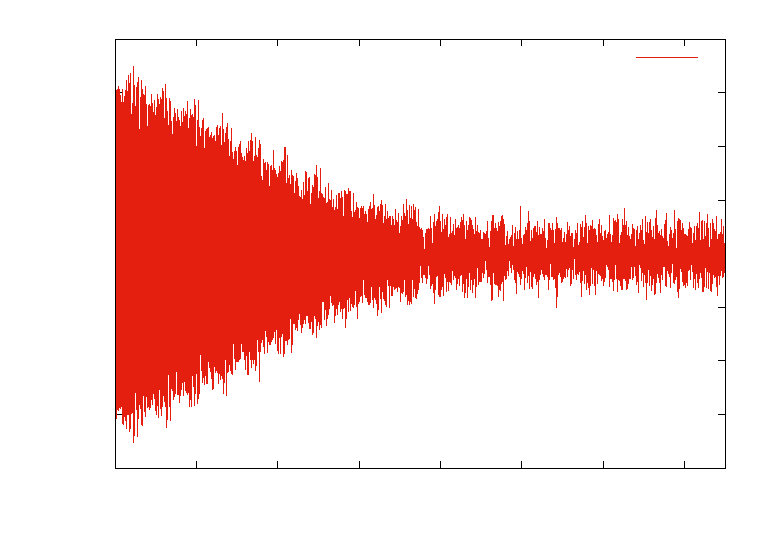
\includegraphics{plots/PulsandcollectValesignal}}%
    \gplfronttext
  \end{picture}%
\endgroup

    \caption[]{Zeige Beispiel wie alles abläuft und danach nur noch ergebnisse}
    \label{fig:PulsandcollectValesignal}
\end{figure}








autoshimm erklären was abging. ergebnisse zeigen. Wie funktioniert verfahren.

\begin{figure}[ht]
    \centering
    % GNUPLOT: LaTeX picture with Postscript
\begingroup
  % Encoding inside the plot.  In the header of your document, this encoding
  % should to defined, e.g., by using
  % \usepackage[cp1252,<other encodings>]{inputenc}
  \inputencoding{cp1252}%
  \makeatletter
  \providecommand\color[2][]{%
    \GenericError{(gnuplot) \space\space\space\@spaces}{%
      Package color not loaded in conjunction with
      terminal option `colourtext'%
    }{See the gnuplot documentation for explanation.%
    }{Either use 'blacktext' in gnuplot or load the package
      color.sty in LaTeX.}%
    \renewcommand\color[2][]{}%
  }%
  \providecommand\includegraphics[2][]{%
    \GenericError{(gnuplot) \space\space\space\@spaces}{%
      Package graphicx or graphics not loaded%
    }{See the gnuplot documentation for explanation.%
    }{The gnuplot epslatex terminal needs graphicx.sty or graphics.sty.}%
    \renewcommand\includegraphics[2][]{}%
  }%
  \providecommand\rotatebox[2]{#2}%
  \@ifundefined{ifGPcolor}{%
    \newif\ifGPcolor
    \GPcolorfalse
  }{}%
  \@ifundefined{ifGPblacktext}{%
    \newif\ifGPblacktext
    \GPblacktexttrue
  }{}%
  % define a \g@addto@macro without @ in the name:
  \let\gplgaddtomacro\g@addto@macro
  % define empty templates for all commands taking text:
  \gdef\gplbacktext{}%
  \gdef\gplfronttext{}%
  \makeatother
  \ifGPblacktext
    % no textcolor at all
    \def\colorrgb#1{}%
    \def\colorgray#1{}%
  \else
    % gray or color?
    \ifGPcolor
      \def\colorrgb#1{\color[rgb]{#1}}%
      \def\colorgray#1{\color[gray]{#1}}%
      \expandafter\def\csname LTw\endcsname{\color{white}}%
      \expandafter\def\csname LTb\endcsname{\color{black}}%
      \expandafter\def\csname LTa\endcsname{\color{black}}%
      \expandafter\def\csname LT0\endcsname{\color[rgb]{1,0,0}}%
      \expandafter\def\csname LT1\endcsname{\color[rgb]{0,1,0}}%
      \expandafter\def\csname LT2\endcsname{\color[rgb]{0,0,1}}%
      \expandafter\def\csname LT3\endcsname{\color[rgb]{1,0,1}}%
      \expandafter\def\csname LT4\endcsname{\color[rgb]{0,1,1}}%
      \expandafter\def\csname LT5\endcsname{\color[rgb]{1,1,0}}%
      \expandafter\def\csname LT6\endcsname{\color[rgb]{0,0,0}}%
      \expandafter\def\csname LT7\endcsname{\color[rgb]{1,0.3,0}}%
      \expandafter\def\csname LT8\endcsname{\color[rgb]{0.5,0.5,0.5}}%
    \else
      % gray
      \def\colorrgb#1{\color{black}}%
      \def\colorgray#1{\color[gray]{#1}}%
      \expandafter\def\csname LTw\endcsname{\color{white}}%
      \expandafter\def\csname LTb\endcsname{\color{black}}%
      \expandafter\def\csname LTa\endcsname{\color{black}}%
      \expandafter\def\csname LT0\endcsname{\color{black}}%
      \expandafter\def\csname LT1\endcsname{\color{black}}%
      \expandafter\def\csname LT2\endcsname{\color{black}}%
      \expandafter\def\csname LT3\endcsname{\color{black}}%
      \expandafter\def\csname LT4\endcsname{\color{black}}%
      \expandafter\def\csname LT5\endcsname{\color{black}}%
      \expandafter\def\csname LT6\endcsname{\color{black}}%
      \expandafter\def\csname LT7\endcsname{\color{black}}%
      \expandafter\def\csname LT8\endcsname{\color{black}}%
    \fi
  \fi
    \setlength{\unitlength}{0.0500bp}%
    \ifx\gptboxheight\undefined%
      \newlength{\gptboxheight}%
      \newlength{\gptboxwidth}%
      \newsavebox{\gptboxtext}%
    \fi%
    \setlength{\fboxrule}{0.5pt}%
    \setlength{\fboxsep}{1pt}%
\begin{picture}(7200.00,5040.00)%
    \gplgaddtomacro\gplbacktext{%
      \csname LTb\endcsname%%
      \put(946,704){\makebox(0,0)[r]{\strut{}$1500$}}%
      \put(946,1527){\makebox(0,0)[r]{\strut{}$2000$}}%
      \put(946,2350){\makebox(0,0)[r]{\strut{}$2500$}}%
      \put(946,3173){\makebox(0,0)[r]{\strut{}$3000$}}%
      \put(946,3996){\makebox(0,0)[r]{\strut{}$3500$}}%
      \put(946,4819){\makebox(0,0)[r]{\strut{}$4000$}}%
      \put(1794,484){\makebox(0,0){\strut{}$6$}}%
      \put(2688,484){\makebox(0,0){\strut{}$8$}}%
      \put(3583,484){\makebox(0,0){\strut{}$10$}}%
      \put(4477,484){\makebox(0,0){\strut{}$12$}}%
      \put(5372,484){\makebox(0,0){\strut{}$14$}}%
      \put(6266,484){\makebox(0,0){\strut{}$16$}}%
    }%
    \gplgaddtomacro\gplfronttext{%
      \csname LTb\endcsname%%
      \put(209,2761){\rotatebox{-270}{\makebox(0,0){\strut{}Frequency $\si{\hertz}$}}}%
      \put(3940,154){\makebox(0,0){\strut{}Capacity in $\si{\nano \farad}$}}%
      \csname LTb\endcsname%%
      \put(5816,4646){\makebox(0,0)[r]{\strut{}measured resonance frequency}}%
      \csname LTb\endcsname%%
      \put(5816,4426){\makebox(0,0)[r]{\strut{}calculated resonance frequency}}%
    }%
    \gplbacktext
    \put(0,0){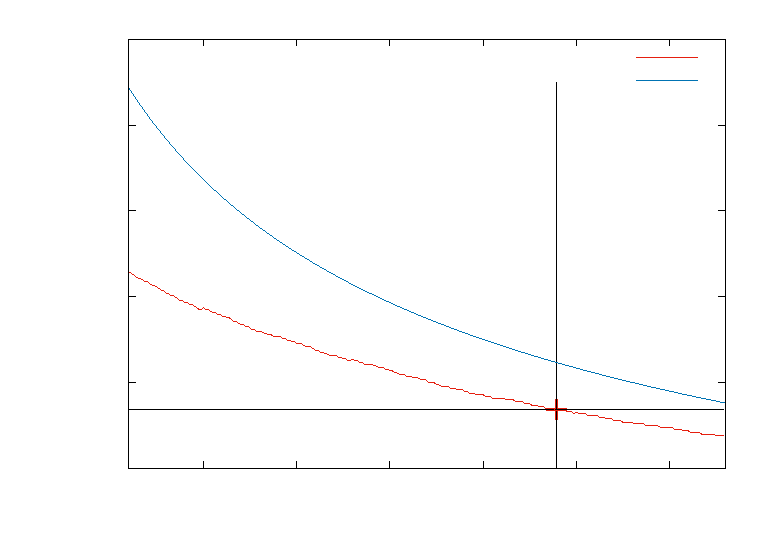
\includegraphics{plots/Coilanalyse}}%
    \gplfronttext
  \end{picture}%
\endgroup

    \caption[]{Wert punkt machen lamorfrequenz. Wieso genau 1834?????? grafik weil schauen wo resonanzfrequenz. Bei Lamorfrequenz Kapazität ablesen. UNsiherheit aus png bild. }
    \label{fig:Coilanalyse}
\end{figure}



\begin{figure}[ht]
    \centering
    % GNUPLOT: LaTeX picture with Postscript
\begingroup
  % Encoding inside the plot.  In the header of your document, this encoding
  % should to defined, e.g., by using
  % \usepackage[cp1252,<other encodings>]{inputenc}
  \inputencoding{cp1252}%
  \makeatletter
  \providecommand\color[2][]{%
    \GenericError{(gnuplot) \space\space\space\@spaces}{%
      Package color not loaded in conjunction with
      terminal option `colourtext'%
    }{See the gnuplot documentation for explanation.%
    }{Either use 'blacktext' in gnuplot or load the package
      color.sty in LaTeX.}%
    \renewcommand\color[2][]{}%
  }%
  \providecommand\includegraphics[2][]{%
    \GenericError{(gnuplot) \space\space\space\@spaces}{%
      Package graphicx or graphics not loaded%
    }{See the gnuplot documentation for explanation.%
    }{The gnuplot epslatex terminal needs graphicx.sty or graphics.sty.}%
    \renewcommand\includegraphics[2][]{}%
  }%
  \providecommand\rotatebox[2]{#2}%
  \@ifundefined{ifGPcolor}{%
    \newif\ifGPcolor
    \GPcolorfalse
  }{}%
  \@ifundefined{ifGPblacktext}{%
    \newif\ifGPblacktext
    \GPblacktexttrue
  }{}%
  % define a \g@addto@macro without @ in the name:
  \let\gplgaddtomacro\g@addto@macro
  % define empty templates for all commands taking text:
  \gdef\gplbacktext{}%
  \gdef\gplfronttext{}%
  \makeatother
  \ifGPblacktext
    % no textcolor at all
    \def\colorrgb#1{}%
    \def\colorgray#1{}%
  \else
    % gray or color?
    \ifGPcolor
      \def\colorrgb#1{\color[rgb]{#1}}%
      \def\colorgray#1{\color[gray]{#1}}%
      \expandafter\def\csname LTw\endcsname{\color{white}}%
      \expandafter\def\csname LTb\endcsname{\color{black}}%
      \expandafter\def\csname LTa\endcsname{\color{black}}%
      \expandafter\def\csname LT0\endcsname{\color[rgb]{1,0,0}}%
      \expandafter\def\csname LT1\endcsname{\color[rgb]{0,1,0}}%
      \expandafter\def\csname LT2\endcsname{\color[rgb]{0,0,1}}%
      \expandafter\def\csname LT3\endcsname{\color[rgb]{1,0,1}}%
      \expandafter\def\csname LT4\endcsname{\color[rgb]{0,1,1}}%
      \expandafter\def\csname LT5\endcsname{\color[rgb]{1,1,0}}%
      \expandafter\def\csname LT6\endcsname{\color[rgb]{0,0,0}}%
      \expandafter\def\csname LT7\endcsname{\color[rgb]{1,0.3,0}}%
      \expandafter\def\csname LT8\endcsname{\color[rgb]{0.5,0.5,0.5}}%
    \else
      % gray
      \def\colorrgb#1{\color{black}}%
      \def\colorgray#1{\color[gray]{#1}}%
      \expandafter\def\csname LTw\endcsname{\color{white}}%
      \expandafter\def\csname LTb\endcsname{\color{black}}%
      \expandafter\def\csname LTa\endcsname{\color{black}}%
      \expandafter\def\csname LT0\endcsname{\color{black}}%
      \expandafter\def\csname LT1\endcsname{\color{black}}%
      \expandafter\def\csname LT2\endcsname{\color{black}}%
      \expandafter\def\csname LT3\endcsname{\color{black}}%
      \expandafter\def\csname LT4\endcsname{\color{black}}%
      \expandafter\def\csname LT5\endcsname{\color{black}}%
      \expandafter\def\csname LT6\endcsname{\color{black}}%
      \expandafter\def\csname LT7\endcsname{\color{black}}%
      \expandafter\def\csname LT8\endcsname{\color{black}}%
    \fi
  \fi
    \setlength{\unitlength}{0.0500bp}%
    \ifx\gptboxheight\undefined%
      \newlength{\gptboxheight}%
      \newlength{\gptboxwidth}%
      \newsavebox{\gptboxtext}%
    \fi%
    \setlength{\fboxrule}{0.5pt}%
    \setlength{\fboxsep}{1pt}%
\begin{picture}(7200.00,5040.00)%
    \gplgaddtomacro\gplbacktext{%
      \csname LTb\endcsname%%
      \put(814,704){\makebox(0,0)[r]{\strut{}$60$}}%
      \put(814,1527){\makebox(0,0)[r]{\strut{}$80$}}%
      \put(814,2350){\makebox(0,0)[r]{\strut{}$100$}}%
      \put(814,3173){\makebox(0,0)[r]{\strut{}$120$}}%
      \put(814,3996){\makebox(0,0)[r]{\strut{}$140$}}%
      \put(814,4819){\makebox(0,0)[r]{\strut{}$160$}}%
      \put(946,484){\makebox(0,0){\strut{}$0$}}%
      \put(1678,484){\makebox(0,0){\strut{}$0.5$}}%
      \put(2410,484){\makebox(0,0){\strut{}$1$}}%
      \put(3142,484){\makebox(0,0){\strut{}$1.5$}}%
      \put(3875,484){\makebox(0,0){\strut{}$2$}}%
      \put(4607,484){\makebox(0,0){\strut{}$2.5$}}%
      \put(5339,484){\makebox(0,0){\strut{}$3$}}%
      \put(6071,484){\makebox(0,0){\strut{}$3.5$}}%
      \put(6803,484){\makebox(0,0){\strut{}$4$}}%
    }%
    \gplgaddtomacro\gplfronttext{%
      \csname LTb\endcsname%%
      \put(209,2761){\rotatebox{-270}{\makebox(0,0){\strut{}FID amplitude}}}%
      \put(3874,154){\makebox(0,0){\strut{}$B_1$ pulse in $\si{}{ms}$}}%
      \csname LTb\endcsname%%
      \put(5816,4646){\makebox(0,0)[r]{\strut{}measured resonance amplitude}}%
    }%
    \gplbacktext
    \put(0,0){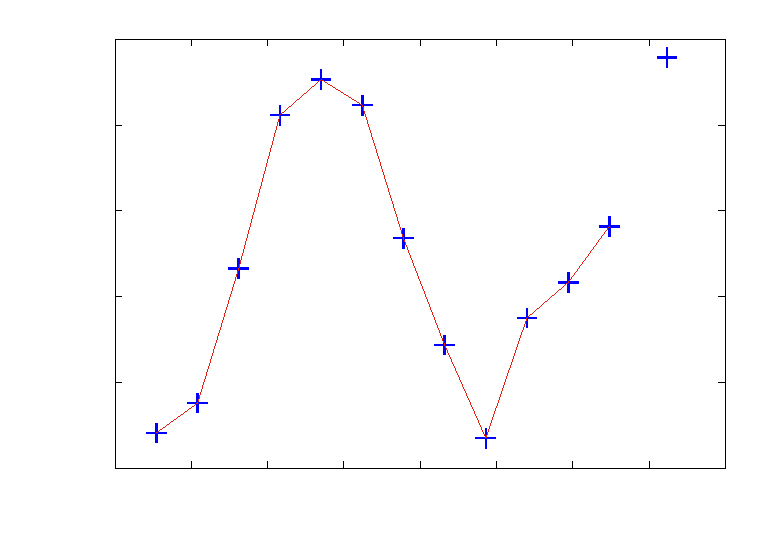
\includegraphics{plots/B1dauer}}%
    \gplfronttext
  \end{picture}%
\endgroup

    \caption[]{Zunahme weil mehr umfllippen. Wieso nimmt wieder ab? antiparallel parallel????????? bei maximum ist es am besten zu messen ca. 1.35ms}
    \label{fig:B1dauer}
\end{figure}
\begin{figure}[ht]
    \centering
    % GNUPLOT: LaTeX picture with Postscript
\begingroup
  % Encoding inside the plot.  In the header of your document, this encoding
  % should to defined, e.g., by using
  % \usepackage[cp1252,<other encodings>]{inputenc}
  \inputencoding{cp1252}%
  \makeatletter
  \providecommand\color[2][]{%
    \GenericError{(gnuplot) \space\space\space\@spaces}{%
      Package color not loaded in conjunction with
      terminal option `colourtext'%
    }{See the gnuplot documentation for explanation.%
    }{Either use 'blacktext' in gnuplot or load the package
      color.sty in LaTeX.}%
    \renewcommand\color[2][]{}%
  }%
  \providecommand\includegraphics[2][]{%
    \GenericError{(gnuplot) \space\space\space\@spaces}{%
      Package graphicx or graphics not loaded%
    }{See the gnuplot documentation for explanation.%
    }{The gnuplot epslatex terminal needs graphicx.sty or graphics.sty.}%
    \renewcommand\includegraphics[2][]{}%
  }%
  \providecommand\rotatebox[2]{#2}%
  \@ifundefined{ifGPcolor}{%
    \newif\ifGPcolor
    \GPcolorfalse
  }{}%
  \@ifundefined{ifGPblacktext}{%
    \newif\ifGPblacktext
    \GPblacktexttrue
  }{}%
  % define a \g@addto@macro without @ in the name:
  \let\gplgaddtomacro\g@addto@macro
  % define empty templates for all commands taking text:
  \gdef\gplbacktext{}%
  \gdef\gplfronttext{}%
  \makeatother
  \ifGPblacktext
    % no textcolor at all
    \def\colorrgb#1{}%
    \def\colorgray#1{}%
  \else
    % gray or color?
    \ifGPcolor
      \def\colorrgb#1{\color[rgb]{#1}}%
      \def\colorgray#1{\color[gray]{#1}}%
      \expandafter\def\csname LTw\endcsname{\color{white}}%
      \expandafter\def\csname LTb\endcsname{\color{black}}%
      \expandafter\def\csname LTa\endcsname{\color{black}}%
      \expandafter\def\csname LT0\endcsname{\color[rgb]{1,0,0}}%
      \expandafter\def\csname LT1\endcsname{\color[rgb]{0,1,0}}%
      \expandafter\def\csname LT2\endcsname{\color[rgb]{0,0,1}}%
      \expandafter\def\csname LT3\endcsname{\color[rgb]{1,0,1}}%
      \expandafter\def\csname LT4\endcsname{\color[rgb]{0,1,1}}%
      \expandafter\def\csname LT5\endcsname{\color[rgb]{1,1,0}}%
      \expandafter\def\csname LT6\endcsname{\color[rgb]{0,0,0}}%
      \expandafter\def\csname LT7\endcsname{\color[rgb]{1,0.3,0}}%
      \expandafter\def\csname LT8\endcsname{\color[rgb]{0.5,0.5,0.5}}%
    \else
      % gray
      \def\colorrgb#1{\color{black}}%
      \def\colorgray#1{\color[gray]{#1}}%
      \expandafter\def\csname LTw\endcsname{\color{white}}%
      \expandafter\def\csname LTb\endcsname{\color{black}}%
      \expandafter\def\csname LTa\endcsname{\color{black}}%
      \expandafter\def\csname LT0\endcsname{\color{black}}%
      \expandafter\def\csname LT1\endcsname{\color{black}}%
      \expandafter\def\csname LT2\endcsname{\color{black}}%
      \expandafter\def\csname LT3\endcsname{\color{black}}%
      \expandafter\def\csname LT4\endcsname{\color{black}}%
      \expandafter\def\csname LT5\endcsname{\color{black}}%
      \expandafter\def\csname LT6\endcsname{\color{black}}%
      \expandafter\def\csname LT7\endcsname{\color{black}}%
      \expandafter\def\csname LT8\endcsname{\color{black}}%
    \fi
  \fi
    \setlength{\unitlength}{0.0500bp}%
    \ifx\gptboxheight\undefined%
      \newlength{\gptboxheight}%
      \newlength{\gptboxwidth}%
      \newsavebox{\gptboxtext}%
    \fi%
    \setlength{\fboxrule}{0.5pt}%
    \setlength{\fboxsep}{1pt}%
\begin{picture}(7200.00,5040.00)%
    \gplgaddtomacro\gplbacktext{%
      \csname LTb\endcsname%%
      \put(682,704){\makebox(0,0)[r]{\strut{}$0$}}%
      \put(682,1161){\makebox(0,0)[r]{\strut{}$10$}}%
      \put(682,1618){\makebox(0,0)[r]{\strut{}$20$}}%
      \put(682,2076){\makebox(0,0)[r]{\strut{}$30$}}%
      \put(682,2533){\makebox(0,0)[r]{\strut{}$40$}}%
      \put(682,2990){\makebox(0,0)[r]{\strut{}$50$}}%
      \put(682,3447){\makebox(0,0)[r]{\strut{}$60$}}%
      \put(682,3905){\makebox(0,0)[r]{\strut{}$70$}}%
      \put(682,4362){\makebox(0,0)[r]{\strut{}$80$}}%
      \put(682,4819){\makebox(0,0)[r]{\strut{}$90$}}%
      \put(814,484){\makebox(0,0){\strut{}$1800$}}%
      \put(2012,484){\makebox(0,0){\strut{}$1820$}}%
      \put(3210,484){\makebox(0,0){\strut{}$1840$}}%
      \put(4407,484){\makebox(0,0){\strut{}$1860$}}%
      \put(5605,484){\makebox(0,0){\strut{}$1880$}}%
      \put(6803,484){\makebox(0,0){\strut{}$1900$}}%
    }%
    \gplgaddtomacro\gplfronttext{%
      \csname LTb\endcsname%%
      \put(209,2761){\rotatebox{-270}{\makebox(0,0){\strut{}Amplitude}}}%
      \put(3808,154){\makebox(0,0){\strut{}frequency in $\si{}{Hz}$}}%
      \csname LTb\endcsname%%
      \put(5816,4646){\makebox(0,0)[r]{\strut{}magnitude spectrum}}%
    }%
    \gplbacktext
    \put(0,0){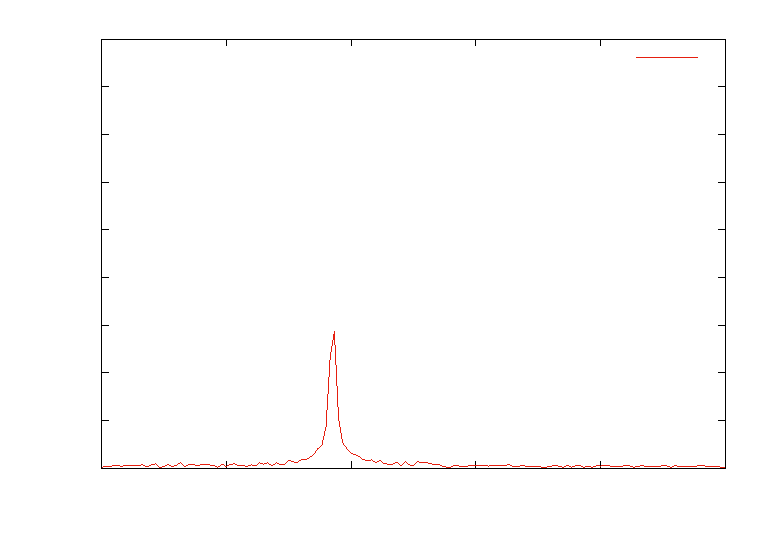
\includegraphics{plots/13.8 puls_and_collect_number_of_delay25ms_Pulseduration0_27ms}}%
    \gplfronttext
  \end{picture}%
\endgroup

    \caption[]{zu kleines signal bei kurzer dauer 0,27ms}
    \label{fig:B1dauer}
\end{figure}
\begin{figure}[ht]
    \centering
    % GNUPLOT: LaTeX picture with Postscript
\begingroup
  % Encoding inside the plot.  In the header of your document, this encoding
  % should to defined, e.g., by using
  % \usepackage[cp1252,<other encodings>]{inputenc}
  \inputencoding{cp1252}%
  \makeatletter
  \providecommand\color[2][]{%
    \GenericError{(gnuplot) \space\space\space\@spaces}{%
      Package color not loaded in conjunction with
      terminal option `colourtext'%
    }{See the gnuplot documentation for explanation.%
    }{Either use 'blacktext' in gnuplot or load the package
      color.sty in LaTeX.}%
    \renewcommand\color[2][]{}%
  }%
  \providecommand\includegraphics[2][]{%
    \GenericError{(gnuplot) \space\space\space\@spaces}{%
      Package graphicx or graphics not loaded%
    }{See the gnuplot documentation for explanation.%
    }{The gnuplot epslatex terminal needs graphicx.sty or graphics.sty.}%
    \renewcommand\includegraphics[2][]{}%
  }%
  \providecommand\rotatebox[2]{#2}%
  \@ifundefined{ifGPcolor}{%
    \newif\ifGPcolor
    \GPcolorfalse
  }{}%
  \@ifundefined{ifGPblacktext}{%
    \newif\ifGPblacktext
    \GPblacktexttrue
  }{}%
  % define a \g@addto@macro without @ in the name:
  \let\gplgaddtomacro\g@addto@macro
  % define empty templates for all commands taking text:
  \gdef\gplbacktext{}%
  \gdef\gplfronttext{}%
  \makeatother
  \ifGPblacktext
    % no textcolor at all
    \def\colorrgb#1{}%
    \def\colorgray#1{}%
  \else
    % gray or color?
    \ifGPcolor
      \def\colorrgb#1{\color[rgb]{#1}}%
      \def\colorgray#1{\color[gray]{#1}}%
      \expandafter\def\csname LTw\endcsname{\color{white}}%
      \expandafter\def\csname LTb\endcsname{\color{black}}%
      \expandafter\def\csname LTa\endcsname{\color{black}}%
      \expandafter\def\csname LT0\endcsname{\color[rgb]{1,0,0}}%
      \expandafter\def\csname LT1\endcsname{\color[rgb]{0,1,0}}%
      \expandafter\def\csname LT2\endcsname{\color[rgb]{0,0,1}}%
      \expandafter\def\csname LT3\endcsname{\color[rgb]{1,0,1}}%
      \expandafter\def\csname LT4\endcsname{\color[rgb]{0,1,1}}%
      \expandafter\def\csname LT5\endcsname{\color[rgb]{1,1,0}}%
      \expandafter\def\csname LT6\endcsname{\color[rgb]{0,0,0}}%
      \expandafter\def\csname LT7\endcsname{\color[rgb]{1,0.3,0}}%
      \expandafter\def\csname LT8\endcsname{\color[rgb]{0.5,0.5,0.5}}%
    \else
      % gray
      \def\colorrgb#1{\color{black}}%
      \def\colorgray#1{\color[gray]{#1}}%
      \expandafter\def\csname LTw\endcsname{\color{white}}%
      \expandafter\def\csname LTb\endcsname{\color{black}}%
      \expandafter\def\csname LTa\endcsname{\color{black}}%
      \expandafter\def\csname LT0\endcsname{\color{black}}%
      \expandafter\def\csname LT1\endcsname{\color{black}}%
      \expandafter\def\csname LT2\endcsname{\color{black}}%
      \expandafter\def\csname LT3\endcsname{\color{black}}%
      \expandafter\def\csname LT4\endcsname{\color{black}}%
      \expandafter\def\csname LT5\endcsname{\color{black}}%
      \expandafter\def\csname LT6\endcsname{\color{black}}%
      \expandafter\def\csname LT7\endcsname{\color{black}}%
      \expandafter\def\csname LT8\endcsname{\color{black}}%
    \fi
  \fi
    \setlength{\unitlength}{0.0500bp}%
    \ifx\gptboxheight\undefined%
      \newlength{\gptboxheight}%
      \newlength{\gptboxwidth}%
      \newsavebox{\gptboxtext}%
    \fi%
    \setlength{\fboxrule}{0.5pt}%
    \setlength{\fboxsep}{1pt}%
\begin{picture}(7200.00,5040.00)%
    \gplgaddtomacro\gplbacktext{%
      \csname LTb\endcsname%%
      \put(682,704){\makebox(0,0)[r]{\strut{}$0$}}%
      \put(682,1161){\makebox(0,0)[r]{\strut{}$10$}}%
      \put(682,1618){\makebox(0,0)[r]{\strut{}$20$}}%
      \put(682,2076){\makebox(0,0)[r]{\strut{}$30$}}%
      \put(682,2533){\makebox(0,0)[r]{\strut{}$40$}}%
      \put(682,2990){\makebox(0,0)[r]{\strut{}$50$}}%
      \put(682,3447){\makebox(0,0)[r]{\strut{}$60$}}%
      \put(682,3905){\makebox(0,0)[r]{\strut{}$70$}}%
      \put(682,4362){\makebox(0,0)[r]{\strut{}$80$}}%
      \put(682,4819){\makebox(0,0)[r]{\strut{}$90$}}%
      \put(814,484){\makebox(0,0){\strut{}$1800$}}%
      \put(2012,484){\makebox(0,0){\strut{}$1820$}}%
      \put(3210,484){\makebox(0,0){\strut{}$1840$}}%
      \put(4407,484){\makebox(0,0){\strut{}$1860$}}%
      \put(5605,484){\makebox(0,0){\strut{}$1880$}}%
      \put(6803,484){\makebox(0,0){\strut{}$1900$}}%
    }%
    \gplgaddtomacro\gplfronttext{%
      \csname LTb\endcsname%%
      \put(209,2761){\rotatebox{-270}{\makebox(0,0){\strut{}Amplitude}}}%
      \put(3808,154){\makebox(0,0){\strut{}frequency in $\si{}{Hz}$}}%
      \csname LTb\endcsname%%
      \put(5816,4646){\makebox(0,0)[r]{\strut{}magnitude spectrum}}%
    }%
    \gplbacktext
    \put(0,0){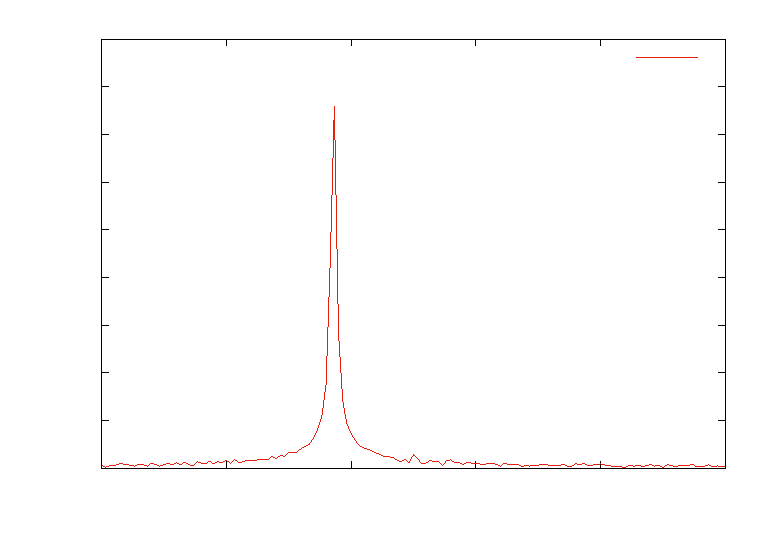
\includegraphics{plots/13.8_puls_and_collect_number_of_delay25ms_Pulseduration1_35ms}}%
    \gplfronttext
  \end{picture}%
\endgroup

    \caption[]{signal ist gut 1,35ms}
    \label{fig:B1dauer}
\end{figure}


\begin{figure}[ht]
    \centering
    % GNUPLOT: LaTeX picture with Postscript
\begingroup
  % Encoding inside the plot.  In the header of your document, this encoding
  % should to defined, e.g., by using
  % \usepackage[cp1252,<other encodings>]{inputenc}
  \inputencoding{cp1252}%
  \makeatletter
  \providecommand\color[2][]{%
    \GenericError{(gnuplot) \space\space\space\@spaces}{%
      Package color not loaded in conjunction with
      terminal option `colourtext'%
    }{See the gnuplot documentation for explanation.%
    }{Either use 'blacktext' in gnuplot or load the package
      color.sty in LaTeX.}%
    \renewcommand\color[2][]{}%
  }%
  \providecommand\includegraphics[2][]{%
    \GenericError{(gnuplot) \space\space\space\@spaces}{%
      Package graphicx or graphics not loaded%
    }{See the gnuplot documentation for explanation.%
    }{The gnuplot epslatex terminal needs graphicx.sty or graphics.sty.}%
    \renewcommand\includegraphics[2][]{}%
  }%
  \providecommand\rotatebox[2]{#2}%
  \@ifundefined{ifGPcolor}{%
    \newif\ifGPcolor
    \GPcolorfalse
  }{}%
  \@ifundefined{ifGPblacktext}{%
    \newif\ifGPblacktext
    \GPblacktexttrue
  }{}%
  % define a \g@addto@macro without @ in the name:
  \let\gplgaddtomacro\g@addto@macro
  % define empty templates for all commands taking text:
  \gdef\gplbacktext{}%
  \gdef\gplfronttext{}%
  \makeatother
  \ifGPblacktext
    % no textcolor at all
    \def\colorrgb#1{}%
    \def\colorgray#1{}%
  \else
    % gray or color?
    \ifGPcolor
      \def\colorrgb#1{\color[rgb]{#1}}%
      \def\colorgray#1{\color[gray]{#1}}%
      \expandafter\def\csname LTw\endcsname{\color{white}}%
      \expandafter\def\csname LTb\endcsname{\color{black}}%
      \expandafter\def\csname LTa\endcsname{\color{black}}%
      \expandafter\def\csname LT0\endcsname{\color[rgb]{1,0,0}}%
      \expandafter\def\csname LT1\endcsname{\color[rgb]{0,1,0}}%
      \expandafter\def\csname LT2\endcsname{\color[rgb]{0,0,1}}%
      \expandafter\def\csname LT3\endcsname{\color[rgb]{1,0,1}}%
      \expandafter\def\csname LT4\endcsname{\color[rgb]{0,1,1}}%
      \expandafter\def\csname LT5\endcsname{\color[rgb]{1,1,0}}%
      \expandafter\def\csname LT6\endcsname{\color[rgb]{0,0,0}}%
      \expandafter\def\csname LT7\endcsname{\color[rgb]{1,0.3,0}}%
      \expandafter\def\csname LT8\endcsname{\color[rgb]{0.5,0.5,0.5}}%
    \else
      % gray
      \def\colorrgb#1{\color{black}}%
      \def\colorgray#1{\color[gray]{#1}}%
      \expandafter\def\csname LTw\endcsname{\color{white}}%
      \expandafter\def\csname LTb\endcsname{\color{black}}%
      \expandafter\def\csname LTa\endcsname{\color{black}}%
      \expandafter\def\csname LT0\endcsname{\color{black}}%
      \expandafter\def\csname LT1\endcsname{\color{black}}%
      \expandafter\def\csname LT2\endcsname{\color{black}}%
      \expandafter\def\csname LT3\endcsname{\color{black}}%
      \expandafter\def\csname LT4\endcsname{\color{black}}%
      \expandafter\def\csname LT5\endcsname{\color{black}}%
      \expandafter\def\csname LT6\endcsname{\color{black}}%
      \expandafter\def\csname LT7\endcsname{\color{black}}%
      \expandafter\def\csname LT8\endcsname{\color{black}}%
    \fi
  \fi
    \setlength{\unitlength}{0.0500bp}%
    \ifx\gptboxheight\undefined%
      \newlength{\gptboxheight}%
      \newlength{\gptboxwidth}%
      \newsavebox{\gptboxtext}%
    \fi%
    \setlength{\fboxrule}{0.5pt}%
    \setlength{\fboxsep}{1pt}%
\begin{picture}(7200.00,5040.00)%
    \gplgaddtomacro\gplbacktext{%
      \csname LTb\endcsname%%
      \put(814,704){\makebox(0,0)[r]{\strut{}$0$}}%
      \put(814,1390){\makebox(0,0)[r]{\strut{}$20$}}%
      \put(814,2076){\makebox(0,0)[r]{\strut{}$40$}}%
      \put(814,2762){\makebox(0,0)[r]{\strut{}$60$}}%
      \put(814,3447){\makebox(0,0)[r]{\strut{}$80$}}%
      \put(814,4133){\makebox(0,0)[r]{\strut{}$100$}}%
      \put(814,4819){\makebox(0,0)[r]{\strut{}$120$}}%
      \put(946,484){\makebox(0,0){\strut{}$1650$}}%
      \put(1678,484){\makebox(0,0){\strut{}$1700$}}%
      \put(2410,484){\makebox(0,0){\strut{}$1750$}}%
      \put(3142,484){\makebox(0,0){\strut{}$1800$}}%
      \put(3875,484){\makebox(0,0){\strut{}$1850$}}%
      \put(4607,484){\makebox(0,0){\strut{}$1900$}}%
      \put(5339,484){\makebox(0,0){\strut{}$1950$}}%
      \put(6071,484){\makebox(0,0){\strut{}$2000$}}%
      \put(6803,484){\makebox(0,0){\strut{}$2050$}}%
    }%
    \gplgaddtomacro\gplfronttext{%
      \csname LTb\endcsname%%
      \put(209,2761){\rotatebox{-270}{\makebox(0,0){\strut{}Amplitude}}}%
      \put(3874,154){\makebox(0,0){\strut{}Frequency in $\si{\hertz}$}}%
      \csname LTb\endcsname%%
      \put(5816,4646){\makebox(0,0)[r]{\strut{}magnitude spectrum}}%
    }%
    \gplbacktext
    \put(0,0){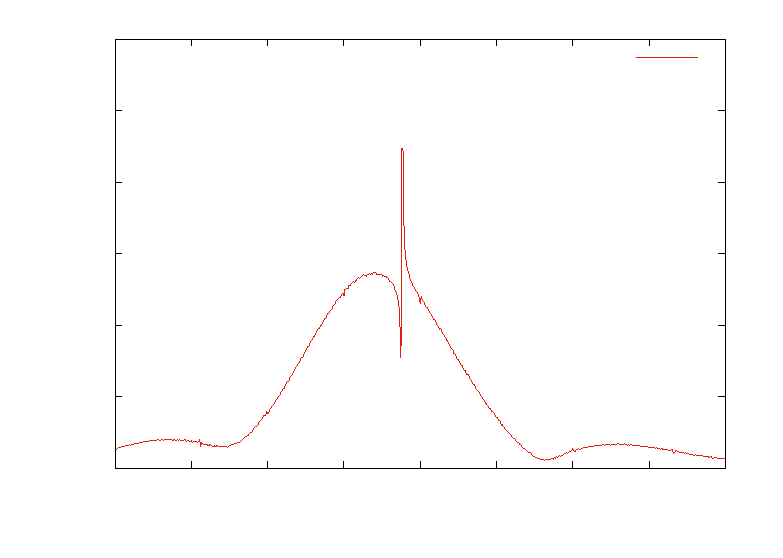
\includegraphics{plots/Pulsandcollect142}}%
    \gplfronttext
  \end{picture}%
\endgroup

    \caption[]{14.2 Kapazität nicht gut im vergleich zu 13.8: sinc funktion rechteckfunktion b1 pulse ist rechteckig.}
    \label{fig:Pulsandcollect142}
\end{figure}
\begin{figure}[ht]
    \centering
    % GNUPLOT: LaTeX picture with Postscript
\begingroup
  % Encoding inside the plot.  In the header of your document, this encoding
  % should to defined, e.g., by using
  % \usepackage[cp1252,<other encodings>]{inputenc}
  \inputencoding{cp1252}%
  \makeatletter
  \providecommand\color[2][]{%
    \GenericError{(gnuplot) \space\space\space\@spaces}{%
      Package color not loaded in conjunction with
      terminal option `colourtext'%
    }{See the gnuplot documentation for explanation.%
    }{Either use 'blacktext' in gnuplot or load the package
      color.sty in LaTeX.}%
    \renewcommand\color[2][]{}%
  }%
  \providecommand\includegraphics[2][]{%
    \GenericError{(gnuplot) \space\space\space\@spaces}{%
      Package graphicx or graphics not loaded%
    }{See the gnuplot documentation for explanation.%
    }{The gnuplot epslatex terminal needs graphicx.sty or graphics.sty.}%
    \renewcommand\includegraphics[2][]{}%
  }%
  \providecommand\rotatebox[2]{#2}%
  \@ifundefined{ifGPcolor}{%
    \newif\ifGPcolor
    \GPcolorfalse
  }{}%
  \@ifundefined{ifGPblacktext}{%
    \newif\ifGPblacktext
    \GPblacktexttrue
  }{}%
  % define a \g@addto@macro without @ in the name:
  \let\gplgaddtomacro\g@addto@macro
  % define empty templates for all commands taking text:
  \gdef\gplbacktext{}%
  \gdef\gplfronttext{}%
  \makeatother
  \ifGPblacktext
    % no textcolor at all
    \def\colorrgb#1{}%
    \def\colorgray#1{}%
  \else
    % gray or color?
    \ifGPcolor
      \def\colorrgb#1{\color[rgb]{#1}}%
      \def\colorgray#1{\color[gray]{#1}}%
      \expandafter\def\csname LTw\endcsname{\color{white}}%
      \expandafter\def\csname LTb\endcsname{\color{black}}%
      \expandafter\def\csname LTa\endcsname{\color{black}}%
      \expandafter\def\csname LT0\endcsname{\color[rgb]{1,0,0}}%
      \expandafter\def\csname LT1\endcsname{\color[rgb]{0,1,0}}%
      \expandafter\def\csname LT2\endcsname{\color[rgb]{0,0,1}}%
      \expandafter\def\csname LT3\endcsname{\color[rgb]{1,0,1}}%
      \expandafter\def\csname LT4\endcsname{\color[rgb]{0,1,1}}%
      \expandafter\def\csname LT5\endcsname{\color[rgb]{1,1,0}}%
      \expandafter\def\csname LT6\endcsname{\color[rgb]{0,0,0}}%
      \expandafter\def\csname LT7\endcsname{\color[rgb]{1,0.3,0}}%
      \expandafter\def\csname LT8\endcsname{\color[rgb]{0.5,0.5,0.5}}%
    \else
      % gray
      \def\colorrgb#1{\color{black}}%
      \def\colorgray#1{\color[gray]{#1}}%
      \expandafter\def\csname LTw\endcsname{\color{white}}%
      \expandafter\def\csname LTb\endcsname{\color{black}}%
      \expandafter\def\csname LTa\endcsname{\color{black}}%
      \expandafter\def\csname LT0\endcsname{\color{black}}%
      \expandafter\def\csname LT1\endcsname{\color{black}}%
      \expandafter\def\csname LT2\endcsname{\color{black}}%
      \expandafter\def\csname LT3\endcsname{\color{black}}%
      \expandafter\def\csname LT4\endcsname{\color{black}}%
      \expandafter\def\csname LT5\endcsname{\color{black}}%
      \expandafter\def\csname LT6\endcsname{\color{black}}%
      \expandafter\def\csname LT7\endcsname{\color{black}}%
      \expandafter\def\csname LT8\endcsname{\color{black}}%
    \fi
  \fi
    \setlength{\unitlength}{0.0500bp}%
    \ifx\gptboxheight\undefined%
      \newlength{\gptboxheight}%
      \newlength{\gptboxwidth}%
      \newsavebox{\gptboxtext}%
    \fi%
    \setlength{\fboxrule}{0.5pt}%
    \setlength{\fboxsep}{1pt}%
\begin{picture}(7200.00,5040.00)%
    \gplgaddtomacro\gplbacktext{%
      \csname LTb\endcsname%%
      \put(814,704){\makebox(0,0)[r]{\strut{}$0$}}%
      \put(814,1390){\makebox(0,0)[r]{\strut{}$20$}}%
      \put(814,2076){\makebox(0,0)[r]{\strut{}$40$}}%
      \put(814,2762){\makebox(0,0)[r]{\strut{}$60$}}%
      \put(814,3447){\makebox(0,0)[r]{\strut{}$80$}}%
      \put(814,4133){\makebox(0,0)[r]{\strut{}$100$}}%
      \put(814,4819){\makebox(0,0)[r]{\strut{}$120$}}%
      \put(946,484){\makebox(0,0){\strut{}$1650$}}%
      \put(1678,484){\makebox(0,0){\strut{}$1700$}}%
      \put(2410,484){\makebox(0,0){\strut{}$1750$}}%
      \put(3142,484){\makebox(0,0){\strut{}$1800$}}%
      \put(3875,484){\makebox(0,0){\strut{}$1850$}}%
      \put(4607,484){\makebox(0,0){\strut{}$1900$}}%
      \put(5339,484){\makebox(0,0){\strut{}$1950$}}%
      \put(6071,484){\makebox(0,0){\strut{}$2000$}}%
      \put(6803,484){\makebox(0,0){\strut{}$2050$}}%
    }%
    \gplgaddtomacro\gplfronttext{%
      \csname LTb\endcsname%%
      \put(209,2761){\rotatebox{-270}{\makebox(0,0){\strut{}Amplitude}}}%
      \put(3874,154){\makebox(0,0){\strut{}Frequency in $\si{\hertz}$}}%
      \csname LTb\endcsname%%
      \put(5816,4646){\makebox(0,0)[r]{\strut{}capacity $\SI{13.8}{\nano \farad}$}}%
      \csname LTb\endcsname%%
      \put(5816,4426){\makebox(0,0)[r]{\strut{}capacity $\SI{14.2}{\nano \farad}$}}%
    }%
    \gplbacktext
    \put(0,0){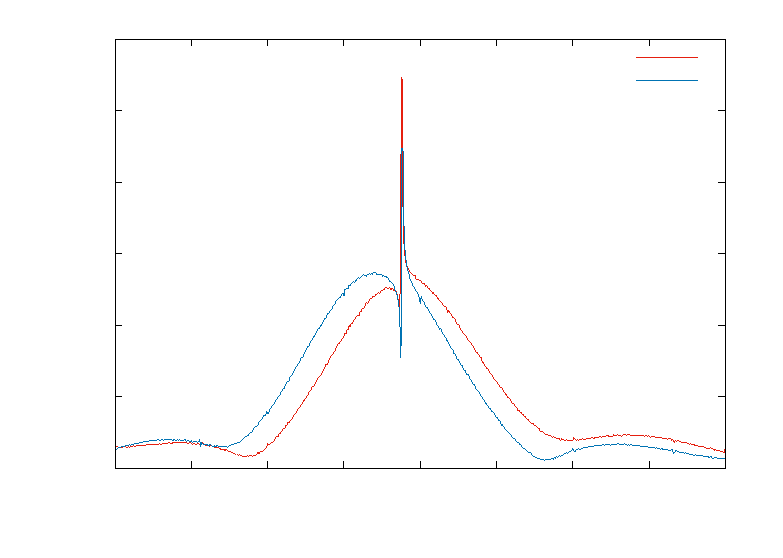
\includegraphics{plots/Pulsandcollect138}}%
    \gplfronttext
  \end{picture}%
\endgroup

    \caption[]{14.2 Kapazität nicht gut im vergleich zu 13.8. signal ist außerdem auch stärker.}
    \label{fig:Pulsandcollect142}
\end{figure}


\begin{figure}[ht]
    \centering
    % GNUPLOT: LaTeX picture with Postscript
\begingroup
  % Encoding inside the plot.  In the header of your document, this encoding
  % should to defined, e.g., by using
  % \usepackage[cp1252,<other encodings>]{inputenc}
  \inputencoding{cp1252}%
  \makeatletter
  \providecommand\color[2][]{%
    \GenericError{(gnuplot) \space\space\space\@spaces}{%
      Package color not loaded in conjunction with
      terminal option `colourtext'%
    }{See the gnuplot documentation for explanation.%
    }{Either use 'blacktext' in gnuplot or load the package
      color.sty in LaTeX.}%
    \renewcommand\color[2][]{}%
  }%
  \providecommand\includegraphics[2][]{%
    \GenericError{(gnuplot) \space\space\space\@spaces}{%
      Package graphicx or graphics not loaded%
    }{See the gnuplot documentation for explanation.%
    }{The gnuplot epslatex terminal needs graphicx.sty or graphics.sty.}%
    \renewcommand\includegraphics[2][]{}%
  }%
  \providecommand\rotatebox[2]{#2}%
  \@ifundefined{ifGPcolor}{%
    \newif\ifGPcolor
    \GPcolorfalse
  }{}%
  \@ifundefined{ifGPblacktext}{%
    \newif\ifGPblacktext
    \GPblacktexttrue
  }{}%
  % define a \g@addto@macro without @ in the name:
  \let\gplgaddtomacro\g@addto@macro
  % define empty templates for all commands taking text:
  \gdef\gplbacktext{}%
  \gdef\gplfronttext{}%
  \makeatother
  \ifGPblacktext
    % no textcolor at all
    \def\colorrgb#1{}%
    \def\colorgray#1{}%
  \else
    % gray or color?
    \ifGPcolor
      \def\colorrgb#1{\color[rgb]{#1}}%
      \def\colorgray#1{\color[gray]{#1}}%
      \expandafter\def\csname LTw\endcsname{\color{white}}%
      \expandafter\def\csname LTb\endcsname{\color{black}}%
      \expandafter\def\csname LTa\endcsname{\color{black}}%
      \expandafter\def\csname LT0\endcsname{\color[rgb]{1,0,0}}%
      \expandafter\def\csname LT1\endcsname{\color[rgb]{0,1,0}}%
      \expandafter\def\csname LT2\endcsname{\color[rgb]{0,0,1}}%
      \expandafter\def\csname LT3\endcsname{\color[rgb]{1,0,1}}%
      \expandafter\def\csname LT4\endcsname{\color[rgb]{0,1,1}}%
      \expandafter\def\csname LT5\endcsname{\color[rgb]{1,1,0}}%
      \expandafter\def\csname LT6\endcsname{\color[rgb]{0,0,0}}%
      \expandafter\def\csname LT7\endcsname{\color[rgb]{1,0.3,0}}%
      \expandafter\def\csname LT8\endcsname{\color[rgb]{0.5,0.5,0.5}}%
    \else
      % gray
      \def\colorrgb#1{\color{black}}%
      \def\colorgray#1{\color[gray]{#1}}%
      \expandafter\def\csname LTw\endcsname{\color{white}}%
      \expandafter\def\csname LTb\endcsname{\color{black}}%
      \expandafter\def\csname LTa\endcsname{\color{black}}%
      \expandafter\def\csname LT0\endcsname{\color{black}}%
      \expandafter\def\csname LT1\endcsname{\color{black}}%
      \expandafter\def\csname LT2\endcsname{\color{black}}%
      \expandafter\def\csname LT3\endcsname{\color{black}}%
      \expandafter\def\csname LT4\endcsname{\color{black}}%
      \expandafter\def\csname LT5\endcsname{\color{black}}%
      \expandafter\def\csname LT6\endcsname{\color{black}}%
      \expandafter\def\csname LT7\endcsname{\color{black}}%
      \expandafter\def\csname LT8\endcsname{\color{black}}%
    \fi
  \fi
    \setlength{\unitlength}{0.0500bp}%
    \ifx\gptboxheight\undefined%
      \newlength{\gptboxheight}%
      \newlength{\gptboxwidth}%
      \newsavebox{\gptboxtext}%
    \fi%
    \setlength{\fboxrule}{0.5pt}%
    \setlength{\fboxsep}{1pt}%
\begin{picture}(7200.00,5040.00)%
    \gplgaddtomacro\gplbacktext{%
      \csname LTb\endcsname%%
      \put(682,704){\makebox(0,0)[r]{\strut{}$0$}}%
      \put(682,1218){\makebox(0,0)[r]{\strut{}$5$}}%
      \put(682,1733){\makebox(0,0)[r]{\strut{}$10$}}%
      \put(682,2247){\makebox(0,0)[r]{\strut{}$15$}}%
      \put(682,2762){\makebox(0,0)[r]{\strut{}$20$}}%
      \put(682,3276){\makebox(0,0)[r]{\strut{}$25$}}%
      \put(682,3790){\makebox(0,0)[r]{\strut{}$30$}}%
      \put(682,4305){\makebox(0,0)[r]{\strut{}$35$}}%
      \put(682,4819){\makebox(0,0)[r]{\strut{}$40$}}%
      \put(814,484){\makebox(0,0){\strut{}$1800$}}%
      \put(2012,484){\makebox(0,0){\strut{}$1820$}}%
      \put(3210,484){\makebox(0,0){\strut{}$1840$}}%
      \put(4407,484){\makebox(0,0){\strut{}$1860$}}%
      \put(5605,484){\makebox(0,0){\strut{}$1880$}}%
      \put(6803,484){\makebox(0,0){\strut{}$1900$}}%
    }%
    \gplgaddtomacro\gplfronttext{%
      \csname LTb\endcsname%%
      \put(209,2761){\rotatebox{-270}{\makebox(0,0){\strut{}Amplitude}}}%
      \put(3808,154){\makebox(0,0){\strut{}Frequency in $\si{}{Hz}$}}%
      \csname LTb\endcsname%%
      \put(5816,4646){\makebox(0,0)[r]{\strut{}magnitude spectrum}}%
    }%
    \gplbacktext
    \put(0,0){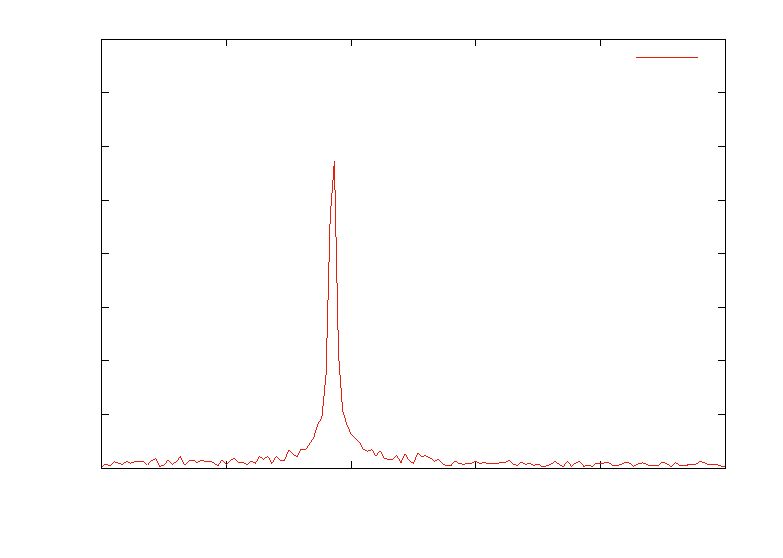
\includegraphics{plots/Pulsandcollect138_delay_25}}%
    \gplfronttext
  \end{picture}%
\endgroup

    \caption[]{größere delay 25ms nur noch wasserstoffsignal. zu dem noch FWHM ausrechnen. integral unter kurve}
    \label{fig:Pulsandcollect142}
\end{figure}
reelles signal, imaginäres signal!!!!!!


T1
bild aus anleitung rein machen und erklären
\begin{figure}[ht]
    \centering
    % GNUPLOT: LaTeX picture with Postscript
\begingroup
  % Encoding inside the plot.  In the header of your document, this encoding
  % should to defined, e.g., by using
  % \usepackage[cp1252,<other encodings>]{inputenc}
  \inputencoding{cp1252}%
  \makeatletter
  \providecommand\color[2][]{%
    \GenericError{(gnuplot) \space\space\space\@spaces}{%
      Package color not loaded in conjunction with
      terminal option `colourtext'%
    }{See the gnuplot documentation for explanation.%
    }{Either use 'blacktext' in gnuplot or load the package
      color.sty in LaTeX.}%
    \renewcommand\color[2][]{}%
  }%
  \providecommand\includegraphics[2][]{%
    \GenericError{(gnuplot) \space\space\space\@spaces}{%
      Package graphicx or graphics not loaded%
    }{See the gnuplot documentation for explanation.%
    }{The gnuplot epslatex terminal needs graphicx.sty or graphics.sty.}%
    \renewcommand\includegraphics[2][]{}%
  }%
  \providecommand\rotatebox[2]{#2}%
  \@ifundefined{ifGPcolor}{%
    \newif\ifGPcolor
    \GPcolorfalse
  }{}%
  \@ifundefined{ifGPblacktext}{%
    \newif\ifGPblacktext
    \GPblacktexttrue
  }{}%
  % define a \g@addto@macro without @ in the name:
  \let\gplgaddtomacro\g@addto@macro
  % define empty templates for all commands taking text:
  \gdef\gplbacktext{}%
  \gdef\gplfronttext{}%
  \makeatother
  \ifGPblacktext
    % no textcolor at all
    \def\colorrgb#1{}%
    \def\colorgray#1{}%
  \else
    % gray or color?
    \ifGPcolor
      \def\colorrgb#1{\color[rgb]{#1}}%
      \def\colorgray#1{\color[gray]{#1}}%
      \expandafter\def\csname LTw\endcsname{\color{white}}%
      \expandafter\def\csname LTb\endcsname{\color{black}}%
      \expandafter\def\csname LTa\endcsname{\color{black}}%
      \expandafter\def\csname LT0\endcsname{\color[rgb]{1,0,0}}%
      \expandafter\def\csname LT1\endcsname{\color[rgb]{0,1,0}}%
      \expandafter\def\csname LT2\endcsname{\color[rgb]{0,0,1}}%
      \expandafter\def\csname LT3\endcsname{\color[rgb]{1,0,1}}%
      \expandafter\def\csname LT4\endcsname{\color[rgb]{0,1,1}}%
      \expandafter\def\csname LT5\endcsname{\color[rgb]{1,1,0}}%
      \expandafter\def\csname LT6\endcsname{\color[rgb]{0,0,0}}%
      \expandafter\def\csname LT7\endcsname{\color[rgb]{1,0.3,0}}%
      \expandafter\def\csname LT8\endcsname{\color[rgb]{0.5,0.5,0.5}}%
    \else
      % gray
      \def\colorrgb#1{\color{black}}%
      \def\colorgray#1{\color[gray]{#1}}%
      \expandafter\def\csname LTw\endcsname{\color{white}}%
      \expandafter\def\csname LTb\endcsname{\color{black}}%
      \expandafter\def\csname LTa\endcsname{\color{black}}%
      \expandafter\def\csname LT0\endcsname{\color{black}}%
      \expandafter\def\csname LT1\endcsname{\color{black}}%
      \expandafter\def\csname LT2\endcsname{\color{black}}%
      \expandafter\def\csname LT3\endcsname{\color{black}}%
      \expandafter\def\csname LT4\endcsname{\color{black}}%
      \expandafter\def\csname LT5\endcsname{\color{black}}%
      \expandafter\def\csname LT6\endcsname{\color{black}}%
      \expandafter\def\csname LT7\endcsname{\color{black}}%
      \expandafter\def\csname LT8\endcsname{\color{black}}%
    \fi
  \fi
    \setlength{\unitlength}{0.0500bp}%
    \ifx\gptboxheight\undefined%
      \newlength{\gptboxheight}%
      \newlength{\gptboxwidth}%
      \newsavebox{\gptboxtext}%
    \fi%
    \setlength{\fboxrule}{0.5pt}%
    \setlength{\fboxsep}{1pt}%
\begin{picture}(7200.00,5040.00)%
    \gplgaddtomacro\gplbacktext{%
      \csname LTb\endcsname%%
      \put(814,704){\makebox(0,0)[r]{\strut{}$0$}}%
      \put(814,1527){\makebox(0,0)[r]{\strut{}$0.2$}}%
      \put(814,2350){\makebox(0,0)[r]{\strut{}$0.4$}}%
      \put(814,3173){\makebox(0,0)[r]{\strut{}$0.6$}}%
      \put(814,3996){\makebox(0,0)[r]{\strut{}$0.8$}}%
      \put(814,4819){\makebox(0,0)[r]{\strut{}$1$}}%
      \put(946,484){\makebox(0,0){\strut{}$0$}}%
      \put(1660,484){\makebox(0,0){\strut{}$500$}}%
      \put(2375,484){\makebox(0,0){\strut{}$1000$}}%
      \put(3089,484){\makebox(0,0){\strut{}$1500$}}%
      \put(3803,484){\makebox(0,0){\strut{}$2000$}}%
      \put(4517,484){\makebox(0,0){\strut{}$2500$}}%
      \put(5232,484){\makebox(0,0){\strut{}$3000$}}%
      \put(5946,484){\makebox(0,0){\strut{}$3500$}}%
      \put(6660,484){\makebox(0,0){\strut{}$4000$}}%
    }%
    \gplgaddtomacro\gplfronttext{%
      \csname LTb\endcsname%%
      \put(209,2761){\rotatebox{-270}{\makebox(0,0){\strut{}Attenuation $\frac{\text{E}}{\text{E}_0}$}}}%
      \put(3874,154){\makebox(0,0){\strut{}Time between pulses $t$ in $\si{\milli \second}$}}%
      \csname LTb\endcsname%%
      \put(5816,4646){\makebox(0,0)[r]{\strut{}measured values}}%
      \csname LTb\endcsname%%
      \put(5816,4426){\makebox(0,0)[r]{\strut{}attenuation-Fit}}%
    }%
    \gplbacktext
    \put(0,0){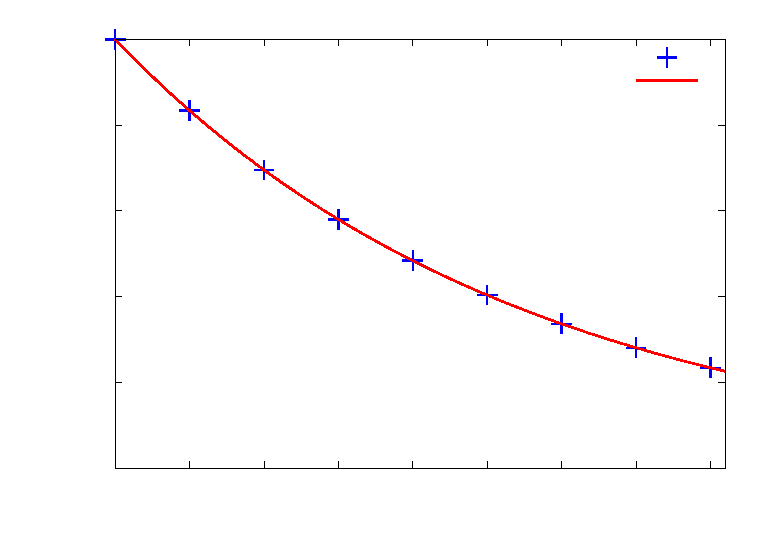
\includegraphics{plots/T1Erdmagnetfeld}}%
    \gplfronttext
  \end{picture}%
\endgroup

    \caption[]{erklären}
    \label{fig:Pulsandcollect142}
\end{figure}

\begin{figure}[ht]
    \centering
    % GNUPLOT: LaTeX picture with Postscript
\begingroup
  % Encoding inside the plot.  In the header of your document, this encoding
  % should to defined, e.g., by using
  % \usepackage[cp1252,<other encodings>]{inputenc}
  \inputencoding{cp1252}%
  \makeatletter
  \providecommand\color[2][]{%
    \GenericError{(gnuplot) \space\space\space\@spaces}{%
      Package color not loaded in conjunction with
      terminal option `colourtext'%
    }{See the gnuplot documentation for explanation.%
    }{Either use 'blacktext' in gnuplot or load the package
      color.sty in LaTeX.}%
    \renewcommand\color[2][]{}%
  }%
  \providecommand\includegraphics[2][]{%
    \GenericError{(gnuplot) \space\space\space\@spaces}{%
      Package graphicx or graphics not loaded%
    }{See the gnuplot documentation for explanation.%
    }{The gnuplot epslatex terminal needs graphicx.sty or graphics.sty.}%
    \renewcommand\includegraphics[2][]{}%
  }%
  \providecommand\rotatebox[2]{#2}%
  \@ifundefined{ifGPcolor}{%
    \newif\ifGPcolor
    \GPcolorfalse
  }{}%
  \@ifundefined{ifGPblacktext}{%
    \newif\ifGPblacktext
    \GPblacktexttrue
  }{}%
  % define a \g@addto@macro without @ in the name:
  \let\gplgaddtomacro\g@addto@macro
  % define empty templates for all commands taking text:
  \gdef\gplbacktext{}%
  \gdef\gplfronttext{}%
  \makeatother
  \ifGPblacktext
    % no textcolor at all
    \def\colorrgb#1{}%
    \def\colorgray#1{}%
  \else
    % gray or color?
    \ifGPcolor
      \def\colorrgb#1{\color[rgb]{#1}}%
      \def\colorgray#1{\color[gray]{#1}}%
      \expandafter\def\csname LTw\endcsname{\color{white}}%
      \expandafter\def\csname LTb\endcsname{\color{black}}%
      \expandafter\def\csname LTa\endcsname{\color{black}}%
      \expandafter\def\csname LT0\endcsname{\color[rgb]{1,0,0}}%
      \expandafter\def\csname LT1\endcsname{\color[rgb]{0,1,0}}%
      \expandafter\def\csname LT2\endcsname{\color[rgb]{0,0,1}}%
      \expandafter\def\csname LT3\endcsname{\color[rgb]{1,0,1}}%
      \expandafter\def\csname LT4\endcsname{\color[rgb]{0,1,1}}%
      \expandafter\def\csname LT5\endcsname{\color[rgb]{1,1,0}}%
      \expandafter\def\csname LT6\endcsname{\color[rgb]{0,0,0}}%
      \expandafter\def\csname LT7\endcsname{\color[rgb]{1,0.3,0}}%
      \expandafter\def\csname LT8\endcsname{\color[rgb]{0.5,0.5,0.5}}%
    \else
      % gray
      \def\colorrgb#1{\color{black}}%
      \def\colorgray#1{\color[gray]{#1}}%
      \expandafter\def\csname LTw\endcsname{\color{white}}%
      \expandafter\def\csname LTb\endcsname{\color{black}}%
      \expandafter\def\csname LTa\endcsname{\color{black}}%
      \expandafter\def\csname LT0\endcsname{\color{black}}%
      \expandafter\def\csname LT1\endcsname{\color{black}}%
      \expandafter\def\csname LT2\endcsname{\color{black}}%
      \expandafter\def\csname LT3\endcsname{\color{black}}%
      \expandafter\def\csname LT4\endcsname{\color{black}}%
      \expandafter\def\csname LT5\endcsname{\color{black}}%
      \expandafter\def\csname LT6\endcsname{\color{black}}%
      \expandafter\def\csname LT7\endcsname{\color{black}}%
      \expandafter\def\csname LT8\endcsname{\color{black}}%
    \fi
  \fi
    \setlength{\unitlength}{0.0500bp}%
    \ifx\gptboxheight\undefined%
      \newlength{\gptboxheight}%
      \newlength{\gptboxwidth}%
      \newsavebox{\gptboxtext}%
    \fi%
    \setlength{\fboxrule}{0.5pt}%
    \setlength{\fboxsep}{1pt}%
\begin{picture}(7200.00,5040.00)%
    \gplgaddtomacro\gplbacktext{%
      \csname LTb\endcsname%%
      \put(814,704){\makebox(0,0)[r]{\strut{}$0$}}%
      \put(814,1527){\makebox(0,0)[r]{\strut{}$0.2$}}%
      \put(814,2350){\makebox(0,0)[r]{\strut{}$0.4$}}%
      \put(814,3173){\makebox(0,0)[r]{\strut{}$0.6$}}%
      \put(814,3996){\makebox(0,0)[r]{\strut{}$0.8$}}%
      \put(814,4819){\makebox(0,0)[r]{\strut{}$1$}}%
      \put(946,484){\makebox(0,0){\strut{}$0$}}%
      \put(1660,484){\makebox(0,0){\strut{}$500$}}%
      \put(2375,484){\makebox(0,0){\strut{}$1000$}}%
      \put(3089,484){\makebox(0,0){\strut{}$1500$}}%
      \put(3803,484){\makebox(0,0){\strut{}$2000$}}%
      \put(4517,484){\makebox(0,0){\strut{}$2500$}}%
      \put(5232,484){\makebox(0,0){\strut{}$3000$}}%
      \put(5946,484){\makebox(0,0){\strut{}$3500$}}%
      \put(6660,484){\makebox(0,0){\strut{}$4000$}}%
    }%
    \gplgaddtomacro\gplfronttext{%
      \csname LTb\endcsname%%
      \put(209,2761){\rotatebox{-270}{\makebox(0,0){\strut{}Attenuation $\frac{\text{E}}{\text{E}_0}$}}}%
      \put(3874,154){\makebox(0,0){\strut{}Time in $\si{\milli \second}$}}%
      \csname LTb\endcsname%%
      \put(5816,4646){\makebox(0,0)[r]{\strut{}measured values$ }}%
      \csname LTb\endcsname%%
      \put(5816,4426){\makebox(0,0)[r]{\strut{}attenuation-Fit}}%
    }%
    \gplbacktext
    \put(0,0){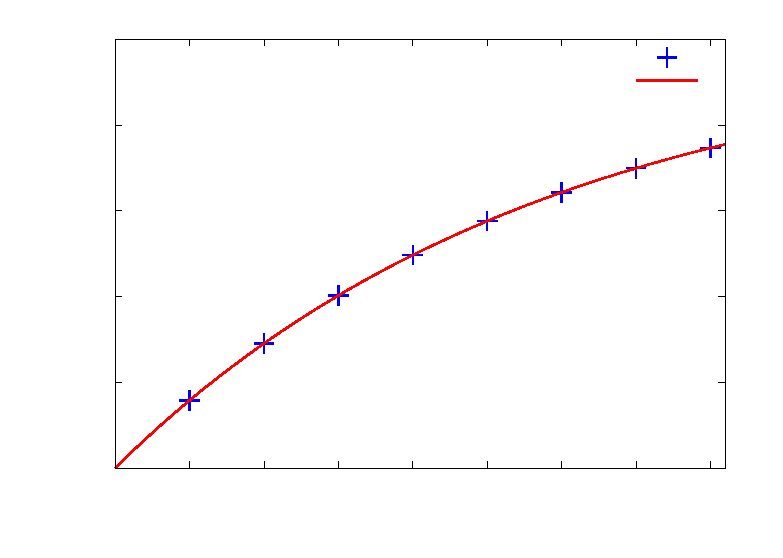
\includegraphics{plots/T1Polarisationsfeldfeld}}%
    \gplfronttext
  \end{picture}%
\endgroup

    \caption[]{erklären. wieso 0.2 überall unterschied}
    \label{fig:Pulsandcollect142}
\end{figure}

hAHN Echo
\begin{figure}[ht]
    \centering
    % GNUPLOT: LaTeX picture with Postscript
\begingroup
  % Encoding inside the plot.  In the header of your document, this encoding
  % should to defined, e.g., by using
  % \usepackage[cp1252,<other encodings>]{inputenc}
  \inputencoding{cp1252}%
  \makeatletter
  \providecommand\color[2][]{%
    \GenericError{(gnuplot) \space\space\space\@spaces}{%
      Package color not loaded in conjunction with
      terminal option `colourtext'%
    }{See the gnuplot documentation for explanation.%
    }{Either use 'blacktext' in gnuplot or load the package
      color.sty in LaTeX.}%
    \renewcommand\color[2][]{}%
  }%
  \providecommand\includegraphics[2][]{%
    \GenericError{(gnuplot) \space\space\space\@spaces}{%
      Package graphicx or graphics not loaded%
    }{See the gnuplot documentation for explanation.%
    }{The gnuplot epslatex terminal needs graphicx.sty or graphics.sty.}%
    \renewcommand\includegraphics[2][]{}%
  }%
  \providecommand\rotatebox[2]{#2}%
  \@ifundefined{ifGPcolor}{%
    \newif\ifGPcolor
    \GPcolorfalse
  }{}%
  \@ifundefined{ifGPblacktext}{%
    \newif\ifGPblacktext
    \GPblacktexttrue
  }{}%
  % define a \g@addto@macro without @ in the name:
  \let\gplgaddtomacro\g@addto@macro
  % define empty templates for all commands taking text:
  \gdef\gplbacktext{}%
  \gdef\gplfronttext{}%
  \makeatother
  \ifGPblacktext
    % no textcolor at all
    \def\colorrgb#1{}%
    \def\colorgray#1{}%
  \else
    % gray or color?
    \ifGPcolor
      \def\colorrgb#1{\color[rgb]{#1}}%
      \def\colorgray#1{\color[gray]{#1}}%
      \expandafter\def\csname LTw\endcsname{\color{white}}%
      \expandafter\def\csname LTb\endcsname{\color{black}}%
      \expandafter\def\csname LTa\endcsname{\color{black}}%
      \expandafter\def\csname LT0\endcsname{\color[rgb]{1,0,0}}%
      \expandafter\def\csname LT1\endcsname{\color[rgb]{0,1,0}}%
      \expandafter\def\csname LT2\endcsname{\color[rgb]{0,0,1}}%
      \expandafter\def\csname LT3\endcsname{\color[rgb]{1,0,1}}%
      \expandafter\def\csname LT4\endcsname{\color[rgb]{0,1,1}}%
      \expandafter\def\csname LT5\endcsname{\color[rgb]{1,1,0}}%
      \expandafter\def\csname LT6\endcsname{\color[rgb]{0,0,0}}%
      \expandafter\def\csname LT7\endcsname{\color[rgb]{1,0.3,0}}%
      \expandafter\def\csname LT8\endcsname{\color[rgb]{0.5,0.5,0.5}}%
    \else
      % gray
      \def\colorrgb#1{\color{black}}%
      \def\colorgray#1{\color[gray]{#1}}%
      \expandafter\def\csname LTw\endcsname{\color{white}}%
      \expandafter\def\csname LTb\endcsname{\color{black}}%
      \expandafter\def\csname LTa\endcsname{\color{black}}%
      \expandafter\def\csname LT0\endcsname{\color{black}}%
      \expandafter\def\csname LT1\endcsname{\color{black}}%
      \expandafter\def\csname LT2\endcsname{\color{black}}%
      \expandafter\def\csname LT3\endcsname{\color{black}}%
      \expandafter\def\csname LT4\endcsname{\color{black}}%
      \expandafter\def\csname LT5\endcsname{\color{black}}%
      \expandafter\def\csname LT6\endcsname{\color{black}}%
      \expandafter\def\csname LT7\endcsname{\color{black}}%
      \expandafter\def\csname LT8\endcsname{\color{black}}%
    \fi
  \fi
    \setlength{\unitlength}{0.0500bp}%
    \ifx\gptboxheight\undefined%
      \newlength{\gptboxheight}%
      \newlength{\gptboxwidth}%
      \newsavebox{\gptboxtext}%
    \fi%
    \setlength{\fboxrule}{0.5pt}%
    \setlength{\fboxsep}{1pt}%
\begin{picture}(7200.00,5040.00)%
    \gplgaddtomacro\gplbacktext{%
      \csname LTb\endcsname%%
      \put(682,704){\makebox(0,0)[r]{\strut{}$0$}}%
      \put(682,1253){\makebox(0,0)[r]{\strut{}$2$}}%
      \put(682,1801){\makebox(0,0)[r]{\strut{}$4$}}%
      \put(682,2350){\makebox(0,0)[r]{\strut{}$6$}}%
      \put(682,2899){\makebox(0,0)[r]{\strut{}$8$}}%
      \put(682,3447){\makebox(0,0)[r]{\strut{}$10$}}%
      \put(682,3996){\makebox(0,0)[r]{\strut{}$12$}}%
      \put(682,4545){\makebox(0,0)[r]{\strut{}$14$}}%
      \put(814,484){\makebox(0,0){\strut{}$1800$}}%
      \put(1563,484){\makebox(0,0){\strut{}$1810$}}%
      \put(2311,484){\makebox(0,0){\strut{}$1820$}}%
      \put(3060,484){\makebox(0,0){\strut{}$1830$}}%
      \put(3809,484){\makebox(0,0){\strut{}$1840$}}%
      \put(4557,484){\makebox(0,0){\strut{}$1850$}}%
      \put(5306,484){\makebox(0,0){\strut{}$1860$}}%
      \put(6054,484){\makebox(0,0){\strut{}$1870$}}%
      \put(6803,484){\makebox(0,0){\strut{}$1880$}}%
    }%
    \gplgaddtomacro\gplfronttext{%
      \csname LTb\endcsname%%
      \put(209,2761){\rotatebox{-270}{\makebox(0,0){\strut{}FID amplitude}}}%
      \put(3808,154){\makebox(0,0){\strut{}Frequency in $\si{}{Hz}$}}%
      \csname LTb\endcsname%%
      \put(5816,4646){\makebox(0,0)[r]{\strut{}shimmin value $x = \si{0}{}}}%
      \csname LTb\endcsname%%
      \put(5816,4426){\makebox(0,0)[r]{\strut{}shimmin value $x = \si{4.95}{}}}%
    }%
    \gplbacktext
    \put(0,0){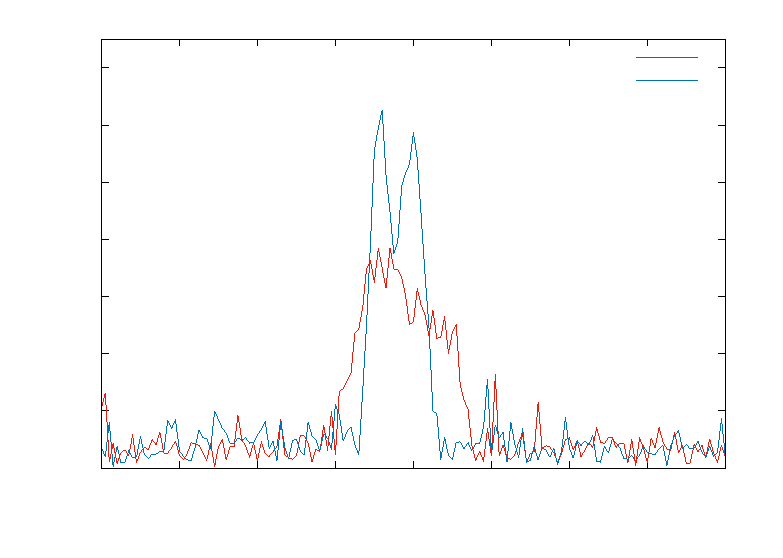
\includegraphics{plots/SpinEcho_4scans_ideal_Repetitiontime_0_shimming_150echo}}%
    \gplfronttext
  \end{picture}%
\endgroup

    \caption[]{wieso signal schwächer vale fragen. integrale bei unterschiedlichen shimming}
    \label{fig:Pulsandcollect142}
\end{figure}
\begin{figure}[ht]
    \centering
    \input{plots/SpinEcho_4scans_ideal_Repetitiontime_4.95xshimming.tex}
    \caption[]{erklären und vale nach signal fragen. integrale bei unterschiedlichen shimming untersuchen??????}
    \label{fig:Pulsandcollect142}
\end{figure}
fragen ob vale daten für verschiedene FIDs bei verschiedenen shimmin hat.
Wo T$_2$ und wo T$_2$stern: T2 bei Pulse and collect normale messung (Narinder fragen): T2stern shimming werte veränder. Spinhahnecho.



CPMG T2

\begin{figure}[ht]
    \centering
    % GNUPLOT: LaTeX picture with Postscript
\begingroup
  % Encoding inside the plot.  In the header of your document, this encoding
  % should to defined, e.g., by using
  % \usepackage[cp1252,<other encodings>]{inputenc}
  \inputencoding{cp1252}%
  \makeatletter
  \providecommand\color[2][]{%
    \GenericError{(gnuplot) \space\space\space\@spaces}{%
      Package color not loaded in conjunction with
      terminal option `colourtext'%
    }{See the gnuplot documentation for explanation.%
    }{Either use 'blacktext' in gnuplot or load the package
      color.sty in LaTeX.}%
    \renewcommand\color[2][]{}%
  }%
  \providecommand\includegraphics[2][]{%
    \GenericError{(gnuplot) \space\space\space\@spaces}{%
      Package graphicx or graphics not loaded%
    }{See the gnuplot documentation for explanation.%
    }{The gnuplot epslatex terminal needs graphicx.sty or graphics.sty.}%
    \renewcommand\includegraphics[2][]{}%
  }%
  \providecommand\rotatebox[2]{#2}%
  \@ifundefined{ifGPcolor}{%
    \newif\ifGPcolor
    \GPcolorfalse
  }{}%
  \@ifundefined{ifGPblacktext}{%
    \newif\ifGPblacktext
    \GPblacktexttrue
  }{}%
  % define a \g@addto@macro without @ in the name:
  \let\gplgaddtomacro\g@addto@macro
  % define empty templates for all commands taking text:
  \gdef\gplbacktext{}%
  \gdef\gplfronttext{}%
  \makeatother
  \ifGPblacktext
    % no textcolor at all
    \def\colorrgb#1{}%
    \def\colorgray#1{}%
  \else
    % gray or color?
    \ifGPcolor
      \def\colorrgb#1{\color[rgb]{#1}}%
      \def\colorgray#1{\color[gray]{#1}}%
      \expandafter\def\csname LTw\endcsname{\color{white}}%
      \expandafter\def\csname LTb\endcsname{\color{black}}%
      \expandafter\def\csname LTa\endcsname{\color{black}}%
      \expandafter\def\csname LT0\endcsname{\color[rgb]{1,0,0}}%
      \expandafter\def\csname LT1\endcsname{\color[rgb]{0,1,0}}%
      \expandafter\def\csname LT2\endcsname{\color[rgb]{0,0,1}}%
      \expandafter\def\csname LT3\endcsname{\color[rgb]{1,0,1}}%
      \expandafter\def\csname LT4\endcsname{\color[rgb]{0,1,1}}%
      \expandafter\def\csname LT5\endcsname{\color[rgb]{1,1,0}}%
      \expandafter\def\csname LT6\endcsname{\color[rgb]{0,0,0}}%
      \expandafter\def\csname LT7\endcsname{\color[rgb]{1,0.3,0}}%
      \expandafter\def\csname LT8\endcsname{\color[rgb]{0.5,0.5,0.5}}%
    \else
      % gray
      \def\colorrgb#1{\color{black}}%
      \def\colorgray#1{\color[gray]{#1}}%
      \expandafter\def\csname LTw\endcsname{\color{white}}%
      \expandafter\def\csname LTb\endcsname{\color{black}}%
      \expandafter\def\csname LTa\endcsname{\color{black}}%
      \expandafter\def\csname LT0\endcsname{\color{black}}%
      \expandafter\def\csname LT1\endcsname{\color{black}}%
      \expandafter\def\csname LT2\endcsname{\color{black}}%
      \expandafter\def\csname LT3\endcsname{\color{black}}%
      \expandafter\def\csname LT4\endcsname{\color{black}}%
      \expandafter\def\csname LT5\endcsname{\color{black}}%
      \expandafter\def\csname LT6\endcsname{\color{black}}%
      \expandafter\def\csname LT7\endcsname{\color{black}}%
      \expandafter\def\csname LT8\endcsname{\color{black}}%
    \fi
  \fi
    \setlength{\unitlength}{0.0500bp}%
    \ifx\gptboxheight\undefined%
      \newlength{\gptboxheight}%
      \newlength{\gptboxwidth}%
      \newsavebox{\gptboxtext}%
    \fi%
    \setlength{\fboxrule}{0.5pt}%
    \setlength{\fboxsep}{1pt}%
\begin{picture}(7200.00,5040.00)%
    \gplgaddtomacro\gplbacktext{%
      \csname LTb\endcsname%%
      \put(814,704){\makebox(0,0)[r]{\strut{}$0$}}%
      \put(814,1527){\makebox(0,0)[r]{\strut{}$0.2$}}%
      \put(814,2350){\makebox(0,0)[r]{\strut{}$0.4$}}%
      \put(814,3173){\makebox(0,0)[r]{\strut{}$0.6$}}%
      \put(814,3996){\makebox(0,0)[r]{\strut{}$0.8$}}%
      \put(814,4819){\makebox(0,0)[r]{\strut{}$1$}}%
      \put(946,484){\makebox(0,0){\strut{}$0$}}%
      \put(1727,484){\makebox(0,0){\strut{}$1000$}}%
      \put(2508,484){\makebox(0,0){\strut{}$2000$}}%
      \put(3289,484){\makebox(0,0){\strut{}$3000$}}%
      \put(4070,484){\makebox(0,0){\strut{}$4000$}}%
      \put(4851,484){\makebox(0,0){\strut{}$5000$}}%
      \put(5632,484){\makebox(0,0){\strut{}$6000$}}%
      \put(6413,484){\makebox(0,0){\strut{}$7000$}}%
    }%
    \gplgaddtomacro\gplfronttext{%
      \csname LTb\endcsname%%
      \put(209,2761){\rotatebox{-270}{\makebox(0,0){\strut{}Attenuation $\frac{\text{E}}{\text{E}_0}$}}}%
      \put(3874,154){\makebox(0,0){\strut{}Time in $\si{\milli \second}$}}%
      \csname LTb\endcsname%%
      \put(5816,4646){\makebox(0,0)[r]{\strut{}measured data}}%
      \csname LTb\endcsname%%
      \put(5816,4426){\makebox(0,0)[r]{\strut{}attenuation Fit}}%
    }%
    \gplbacktext
    \put(0,0){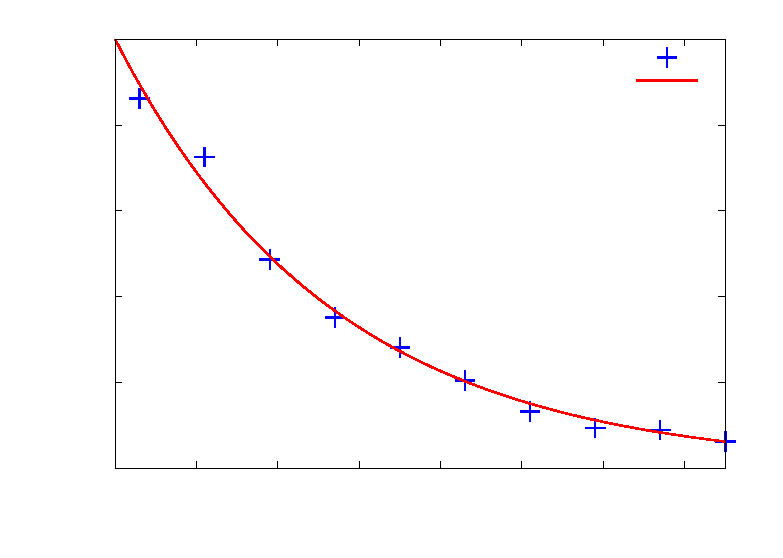
\includegraphics{plots/T2}}%
    \gplfronttext
  \end{picture}%
\endgroup

    \caption[]{wie ging diese verfickte Messung??}
    \label{fig:Pulsandcollect142}
\end{figure}

\begin{figure}[ht]
    \centering
    % GNUPLOT: LaTeX picture with Postscript
\begingroup
  % Encoding inside the plot.  In the header of your document, this encoding
  % should to defined, e.g., by using
  % \usepackage[cp1252,<other encodings>]{inputenc}
  \inputencoding{cp1252}%
  \makeatletter
  \providecommand\color[2][]{%
    \GenericError{(gnuplot) \space\space\space\@spaces}{%
      Package color not loaded in conjunction with
      terminal option `colourtext'%
    }{See the gnuplot documentation for explanation.%
    }{Either use 'blacktext' in gnuplot or load the package
      color.sty in LaTeX.}%
    \renewcommand\color[2][]{}%
  }%
  \providecommand\includegraphics[2][]{%
    \GenericError{(gnuplot) \space\space\space\@spaces}{%
      Package graphicx or graphics not loaded%
    }{See the gnuplot documentation for explanation.%
    }{The gnuplot epslatex terminal needs graphicx.sty or graphics.sty.}%
    \renewcommand\includegraphics[2][]{}%
  }%
  \providecommand\rotatebox[2]{#2}%
  \@ifundefined{ifGPcolor}{%
    \newif\ifGPcolor
    \GPcolorfalse
  }{}%
  \@ifundefined{ifGPblacktext}{%
    \newif\ifGPblacktext
    \GPblacktexttrue
  }{}%
  % define a \g@addto@macro without @ in the name:
  \let\gplgaddtomacro\g@addto@macro
  % define empty templates for all commands taking text:
  \gdef\gplbacktext{}%
  \gdef\gplfronttext{}%
  \makeatother
  \ifGPblacktext
    % no textcolor at all
    \def\colorrgb#1{}%
    \def\colorgray#1{}%
  \else
    % gray or color?
    \ifGPcolor
      \def\colorrgb#1{\color[rgb]{#1}}%
      \def\colorgray#1{\color[gray]{#1}}%
      \expandafter\def\csname LTw\endcsname{\color{white}}%
      \expandafter\def\csname LTb\endcsname{\color{black}}%
      \expandafter\def\csname LTa\endcsname{\color{black}}%
      \expandafter\def\csname LT0\endcsname{\color[rgb]{1,0,0}}%
      \expandafter\def\csname LT1\endcsname{\color[rgb]{0,1,0}}%
      \expandafter\def\csname LT2\endcsname{\color[rgb]{0,0,1}}%
      \expandafter\def\csname LT3\endcsname{\color[rgb]{1,0,1}}%
      \expandafter\def\csname LT4\endcsname{\color[rgb]{0,1,1}}%
      \expandafter\def\csname LT5\endcsname{\color[rgb]{1,1,0}}%
      \expandafter\def\csname LT6\endcsname{\color[rgb]{0,0,0}}%
      \expandafter\def\csname LT7\endcsname{\color[rgb]{1,0.3,0}}%
      \expandafter\def\csname LT8\endcsname{\color[rgb]{0.5,0.5,0.5}}%
    \else
      % gray
      \def\colorrgb#1{\color{black}}%
      \def\colorgray#1{\color[gray]{#1}}%
      \expandafter\def\csname LTw\endcsname{\color{white}}%
      \expandafter\def\csname LTb\endcsname{\color{black}}%
      \expandafter\def\csname LTa\endcsname{\color{black}}%
      \expandafter\def\csname LT0\endcsname{\color{black}}%
      \expandafter\def\csname LT1\endcsname{\color{black}}%
      \expandafter\def\csname LT2\endcsname{\color{black}}%
      \expandafter\def\csname LT3\endcsname{\color{black}}%
      \expandafter\def\csname LT4\endcsname{\color{black}}%
      \expandafter\def\csname LT5\endcsname{\color{black}}%
      \expandafter\def\csname LT6\endcsname{\color{black}}%
      \expandafter\def\csname LT7\endcsname{\color{black}}%
      \expandafter\def\csname LT8\endcsname{\color{black}}%
    \fi
  \fi
    \setlength{\unitlength}{0.0500bp}%
    \ifx\gptboxheight\undefined%
      \newlength{\gptboxheight}%
      \newlength{\gptboxwidth}%
      \newsavebox{\gptboxtext}%
    \fi%
    \setlength{\fboxrule}{0.5pt}%
    \setlength{\fboxsep}{1pt}%
\begin{picture}(7200.00,5040.00)%
    \gplgaddtomacro\gplbacktext{%
      \csname LTb\endcsname%%
      \put(814,704){\makebox(0,0)[r]{\strut{}$0$}}%
      \put(814,1527){\makebox(0,0)[r]{\strut{}$0.2$}}%
      \put(814,2350){\makebox(0,0)[r]{\strut{}$0.4$}}%
      \put(814,3173){\makebox(0,0)[r]{\strut{}$0.6$}}%
      \put(814,3996){\makebox(0,0)[r]{\strut{}$0.8$}}%
      \put(814,4819){\makebox(0,0)[r]{\strut{}$1$}}%
      \put(1754,484){\makebox(0,0){\strut{}$1000$}}%
      \put(2764,484){\makebox(0,0){\strut{}$2000$}}%
      \put(3774,484){\makebox(0,0){\strut{}$3000$}}%
      \put(4783,484){\makebox(0,0){\strut{}$4000$}}%
      \put(5793,484){\makebox(0,0){\strut{}$5000$}}%
      \put(6803,484){\makebox(0,0){\strut{}$6000$}}%
    }%
    \gplgaddtomacro\gplfronttext{%
      \csname LTb\endcsname%%
      \put(209,2761){\rotatebox{-270}{\makebox(0,0){\strut{}Amplitude $\frac{E}{E_0}$}}}%
      \put(3874,154){\makebox(0,0){\strut{}time in $\si{}{ms}$}}%
      \csname LTb\endcsname%%
      \put(5816,4646){\makebox(0,0)[r]{\strut{}the spin-spin relacation dependent from the time with an inhomogene field}}%
      \csname LTb\endcsname%%
      \put(5816,4426){\makebox(0,0)[r]{\strut{}\textsc{Keine Ahnung}-Fit $M(x)=M_0 * exp(-x/T_2)$ with $T_2=\SI[2317.76][milisec]$}}%
    }%
    \gplbacktext
    \put(0,0){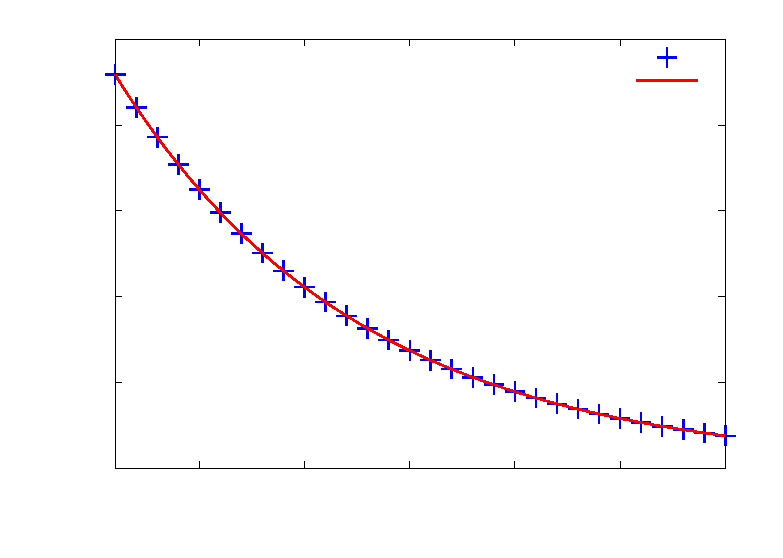
\includegraphics{plots/CPMG0.45shimming}}%
    \gplfronttext
  \end{picture}%
\endgroup

    \caption[]{time domain filter. Schneller, nicht schneller abfall. Mehrere Echos}
    \label{fig:Pulsandcollect142}
\end{figure}
Vale fragen nach signaldaten